%
%	final_report.tex
%
%	Final Report Outline
%
%	John Hughes and Michael Jean
%	University of Manitoba
%

\documentclass[english]{scrreprt}

\KOMAoptions{fontsize=11pt}
\KOMAoptions{paper=letter}

%%% Preamble

%
%	preamble.tex
%
%	Final Report: Document Preamble
%
%	John Hughes and Michael Jean
%	University of Manitoba
%

\usepackage[T1]{fontenc}
\usepackage[utf8x]{inputenc}

\setcounter{secnumdepth}{3}
\setcounter{tocdepth}{3}

\usepackage{amsmath}
\usepackage{array}
\usepackage{babel}
\usepackage{float}
\usepackage[letterpaper]{geometry}
\usepackage{graphicx}
\usepackage{graphics}
\usepackage{lastpage}
\usepackage{tikz}
\usepackage{tikz-timing}[2009/05/15]
\usepackage{subfigure}
\usepackage{tabularx}
\usepackage{array}
\usepackage{flafter,fnpos}
\usepackage{booktabs}
\usepackage{supertabular}
\usepackage{setspace}
\usepackage{indentfirst}

\usepackage[binary]{SIunits}

%\usepackage[square,authoryear,sort&compress]{natbib}
\usepackage[numbers, square, comma, sort&compress]{natbib}

\usepackage{nomencl}
\makenomenclature

\usepackage{fancyhdr}

%%% Set Margins
\setlength{\hoffset}{0.5in}
\oddsidemargin=0pt
\setlength{\topmargin}{0pt}
\setlength{\marginparwidth}{0pt}
\setlength{\marginparsep}{0pt}
\setlength{\textwidth}{6in}
\setlength{\textheight}{600pt}
\setlength{\footskip}{20pt}
\setlength{\headsep}{15pt}

\setlength{\parskip}{\medskipamount}
\makeatletter

% Tikz styles

\usetikzlibrary{shapes,arrows,shadows,calc}

% Define the arm and angle options
\def\myarm{1cm}
\def\myangle{0}
\tikzset{
  arm/.default=1cm,
  arm/.code={\def\myarm{#1}}, % store value in \myarm
  angle/.default=0,
  angle/.code={\def\myangle{#1}} % store value in \myangle
}

% Define the myncbar to path
\tikzset{
    myncbar/.style = {to path={
        % We need to calculate a couple of coordinates to help us draw
        % the path. 
        let
            % Same as (\tikztotarget)++(\myangle:\myarm)
            \p1=($(\tikztotarget)+(\myangle:\myarm)$)
        in
            -- ++(\myangle:\myarm) coordinate (tmp)
            % Find the projection of the (tmp) coordinate
            % on the line from the target to p1
            -- ($(\tikztotarget)!(tmp)!(\p1)$)
            -- (\tikztotarget)\tikztonodes
    }}
}

\tikzstyle{red shiny} = [draw=red!50!black!50, top color=white,bottom color=red!50!black!20, drop shadow]
\tikzstyle{blue shiny} = [draw=blue!50!black!50, top color=white,bottom color=blue!50!black!20, drop shadow]
\tikzstyle{grey shiny} = [draw=gray!50!black!50, top color=white,bottom color=gray!50!black!20, drop shadow]

\tikzstyle{start} = [grey shiny, signal, signal to=east, draw]
\tikzstyle{end} = [grey shiny, signal, signal from=east, draw]
\tikzstyle{decision} = [ blue shiny, diamond, text width=1cm, text badly centered, inner sep=0pt]

\tikzstyle{module} = [ blue shiny, rectangle, very thick]

\tikzstyle{block} = [ red shiny, rectangle,
		      %minimum height=3em,
		      %minimum width=6em,
		      %inner sep=0.5em,
		      text width=2cm,
		      text centered]
\tikzstyle{bus} = [coordinate]
\tikzstyle{input} = [coordinate]
\tikzstyle{output} = [coordinate]

\tikzstyle{small block} = [ red shiny,
		      rectangle,
		      very thick,
		      %minimum height=3em,
		      %minimum width=3em,
		      inner sep=0.5em,
		      text width=1cm,
		      text centered]

\usepackage[
  unicode=true,
  pdfusetitle,
  bookmarks=true,
  bookmarksnumbered=true,
  bookmarksopen=false,
  breaklinks=false,
  pdfborder={0 0 0},
  backref=false,
  colorlinks=false
] {hyperref}

\renewcommand{\baselinestretch}{1.0}

\begin{document}
\pagenumbering{roman}

%%% Title Page

\subject{Design and implementation of an automotive sensor/actuator network for the Formula SAE 2010 vehicle}
\title{Final Report}

\author{John Hughes\\ Michael Jean\\ Group Advisor: Dr. W. Kinsner\\ G27}

\maketitle

%%% Visual Abstract
\vspace*{1in}
\begin{center}
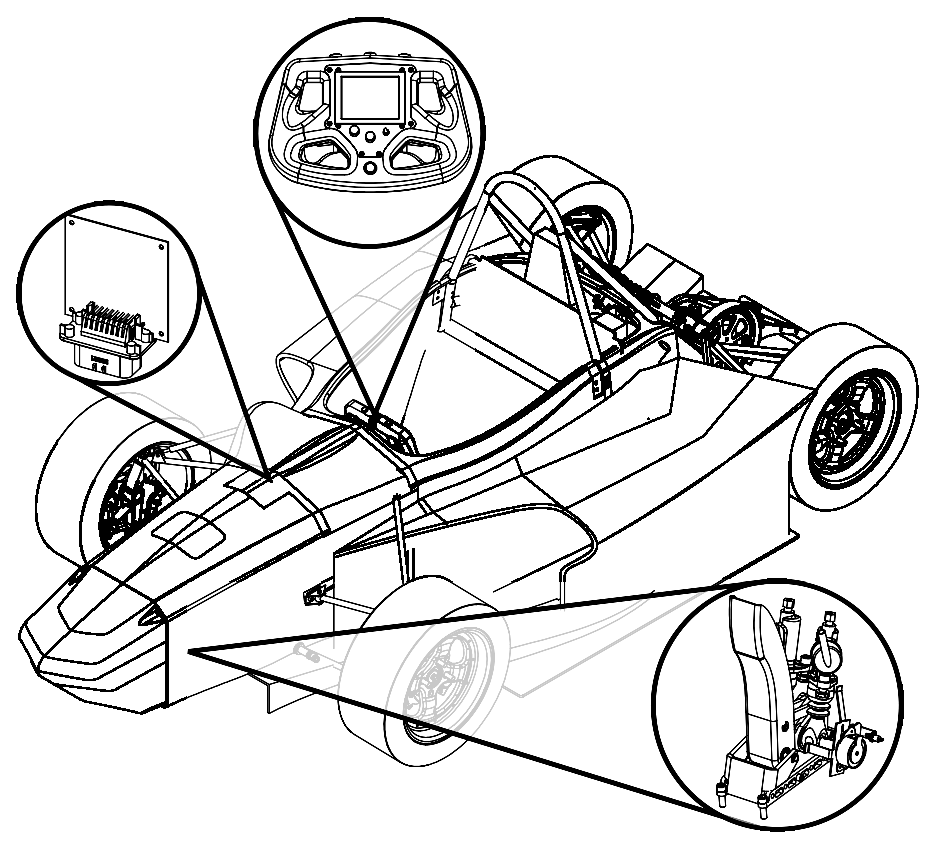
\includegraphics[scale=1]{visual_abstract.eps}
\end{center}
\phantomsection \label{visual_abstract}
\addcontentsline{toc}{chapter}{Visual Abstract}

%%% Set up fancy headers
\pagestyle{fancy}

%%% Add the running title to the left side of the header
\fancyhead[L]{Distributed Sensor/Actuator Network}

\begin{abstract}
\begin{abstract}
A Formula SAE vehicle is a performance car built with the primary goal of ranking highly in the dynamic events at the yearly competitions. The goal of this work is to tackle several distinct issues relating 2010 Formula SAE Vehicle constructed at the University of Manitoba. Specifically: to improve electronic control of the transmission, to control the actuator for an adjustable variable-length air intake plenum, to control the brake bias electronically, to broadcast telemetry data from on-board systems to the pit crew, and to create an easy to use driver interface and dashboard.

The problems were approached with a distributed divide and conquer method. An architecture of four seperate electronic modules was devised: an engine and transmission module, a braking module, a telemetry module and a driver interface module. Each module is designed to communicate with the others as well as with pre-existing modules.

Four working prototype modules were constructed with custom-designed printed circuit boards. All hardware was implemented and debugged. All software for the braking module software was successfully written and tested. Telemetry data was successfully multiplexed and transmitted from the vehicle's two on-board sources to software running on a PC. All low-level driver software for the driver interface module was written and tested. A novel electro-pneumatic transmission actuation scheme was developed and modelled and simulated in Matlab/Simulink.

Final testing of the engine and transmission module, and the braking module was not conducted since the completed SAE vehicle intended for installation was not yet available.
\end{abstract}


\end{abstract}

\chapter*{Contributions}
\addcontentsline{toc}{chapter}{Contributions}
Contributions

\chapter*{Acknowledgements}
\addcontentsline{toc}{chapter}{Acknowledgements}
Acknowledgements

\renewcommand{\contentsname}{Table of Contents}

%%% Shorten the TOC depth
\setcounter{tocdepth}{1}
\tableofcontents{}

\newpage
\phantomsection \label{listoffig}
\addcontentsline{toc}{chapter}{List of Figures}
\listoffigures

\newpage
\phantomsection \label{listoftab}
\addcontentsline{toc}{chapter}{List of Tables}
\listoftables

\newpage
\phantomsection \label{nomenclature}
\addcontentsline{toc}{chapter}{Nomenclature}
\printnomenclature{}

\newpage

\pagenumbering{arabic}
%\setstretch{1.5}

\chapter{Introduction\label{cha:introduction}}

The purpose of this chapter is to provide a broad introduction to the project by first introducing our student group, our motivations for undertaking the project, the scope and definition of the problems we would like to solve, and the strategy undertaken to solve these problems. We will also close with a brief outline of each section in this report.

\section{Formula SAE}

Formula SAE\nomenclature{SAE}{Society of Automotive Engineers} is an engineering student design competition organized by the Society of Automotive Engineers dating back to 1978 \cite{fsaehistory}. Students from the University of Manitoba have participated in the competition almost every year since 1985. The competition consists of designing and constructing a small, open-wheeled, formula-style race car.

The Formula SAE vehicle is a performance car built with the primary goal of doing well in the dynamic events at the yearly competitions. These events test the vehicles' abilities in acceleration, braking, and handling. 

\section{Motivation}

Many of the issues that directly affect the teams' performance at competition relate to driver training, feedback, and the tunability of the car. Most of the mechanical systems on the car must currently be imprecisely hand-tuned, and are packaged in hard to reach places, and require body panels or the seat to be removed for access.

Our overall goal is thus to improve the precision, adjustability, and repeatability of adjustment, of various important mechanical systems in the car, and to improve the efficiency of testing. Highly desirable is a shorter driver-feedback-tuning loop in order to eliminate overshoot and undershoot in tuning, and to avoid other external disturbances.

A second major goal is to improve upon the transmission control systems of previous years' designs.

\section{Problem Definition}

The goal of this work is to tackle several distinct issues on the 2010 Formula SAE Vehicle, specifically:

\begin{itemize}
 \item to improve the electronic control of the transmission;
 \item to introduce an automatically-adjusting variable-length air intake;
 \item to make the brake bias adjustable electronically;
 \item to broadcast telemetry data from on-board systems to the pit crew; and
 \item to create an easy-to-use driver interface.
\end{itemize}

Improving the electronic control of the transmission will decrease the time required to change gears, improve the mechanical reliability of the transmission, and decrease the effort required by the driver to change gears. 

Introducing an automatically adjusting variable-length air intake will widen the peak torque output from the engine. This will improve engine responsiveness and vehicle acceleration.
 
Making the brake bias adjustable electronically will allow on-the-fly bias adjustment, even while the vehicle is in motion. This will eliminate the need for manual adjustment and calibration.
 
Broadcasting telemetry data to the pit crew will allow the team to make decisions regarding the dynamic parameters of the vehicle. This will optimize vehicle performance and provide feedback to the crew regarding the quality of any parameter tuning.

Creating an easy-to-use driver interface will allow the driver to tune the dynamic parameters of the vehicle from a simple interface located on the steering wheel, and will also provide the driver with real-time feedback from the various vehicle sensors. This will allow the driver to optimize the vehicle's dynamic parameters for their own driving style, and keep the driver informed of the vehicle's state without being distracting.
 
\section{Strategy \label{sec:intro_strategy}}

Four networked electronic modules and an electro-pneumatic actuation system will be created to meet the goals outlined in the problem definition. The four modules are:

\begin{itemize}
\item the transmission and engine control module;
\item the brake bias adjustment module;
\item the wireless telemetry module; and
\item the driver interface module.
\end{itemize}

The transmission and engine control module will interface with the electro-pneumatic actuation system to control the transmission. The design and implementation of the system requires several steps:

\begin{enumerate}

\item Absolute requirements and specifications for system parameters are first established. The electromechanical interface linking the control systems and mechanical systems are decided between our group and the mechanical engineers responsible for each respective system. The measurement requirements from the mechanical systems are established and the appropriate sensors are chosen.

\item Appropriate components for the electronic modules are chosen, and the circuits are designed. The schematic of each module is designed and an appropriate printed circuit board is laid out. The boards are manufactured and populated with components. Each board must be tested to ensure all wiring is correct and the functionality of all the components is correct.

\item Firmware for each module must be implemented once the hardware design is finished. Software libraries for various components are written and tested. The libraries are combined with a high-level control algorithm for each module.
 
\item Each module is tested in isolation to ensure proper functionality. 

\item The modules are then interconnected and tested again.

\end{enumerate}

\section{Outline of Thesis}

This thesis is organized into 8 chapters. After this introductory chapter, Ch. \ref{cha:background} provides background information describing the vehicle systems we will interact with, the problems associated with these systems we are attempting to solve, and a description of previous efforts to solve these problems. 

In Ch. \ref{cha:goals} the goals and requirements of the design work will be specified for each of the areas described in Ch. \ref{cha:background}. 

Chapter \ref{cha:design} describes our design to meet these requirements. 

Chapter \ref{cha:implementation} describes our implementation of the design.


\chapter{Background\label{cha:background}}

The 2010 Formula SAE vehicle is essentially made up of five functional systems, namely the \emph{engine}, \emph{transmission}, \emph{braking}, \emph{telemetry}, and \emph{driver interface} systems. The background of these systems is discussed further in this chapter, to provide the reader with the knowledge required to follow the reasoning for our design. The specific vehicle components that interface with the four electronic modules and the electro-pneumatic system are annotated in Fig. \ref{fig:background_overview_topdown}. 

\vspace{1em}
\begin{figure}[H]
\centering
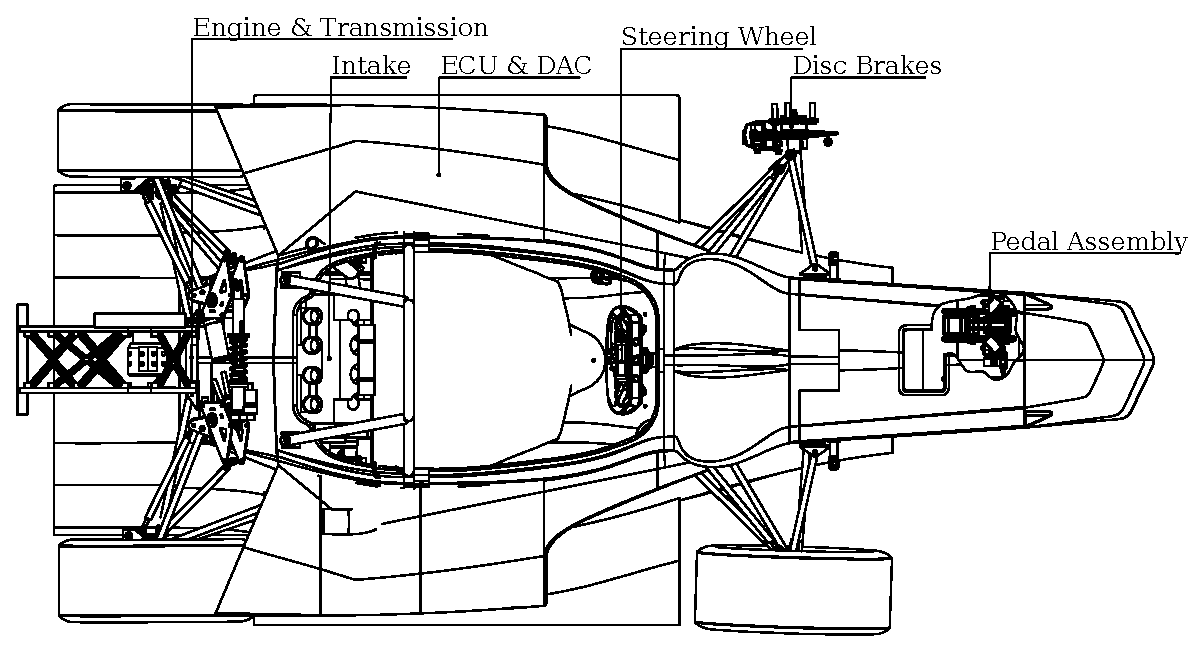
\includegraphics[width=6in,keepaspectratio]{background/figures/background_diagram.eps}
\caption{Top-down view of the 2010 Formula SAE vehicle.}
\label{fig:background_overview_topdown}
\end{figure}

\section{Engine}

\subsection{Overview}

brief {}``what is engine'', honda cbr, etc.

maximise power output (performance application)

torque power curve, etc.

\subsection{ECU}

A specialized third-party component called the \emph{Engine Control Unit} (ECU) controls the fuel injector and spark coil systems that in turn control the combustion cycle of the engine. The particular model of ECU used by the Formula SAE car is the S80Pro from DTAFast \cite{s80pro}. The ECU uses the O$_{2}$, MAP, cam position, and crank position sensors to adjust the fuel injector and spark coil timings. This keeps the engine running smoothly. The ECU features a traction control system that monitors wheel slip and cuts spark and fuel to provide traction when one of the wheels is slipping. The ECU also collects the various sensor readings and makes them available to other electronic devices at a fixed frequency through a shared data bus. 

\begin{figure}[H]
\centering
%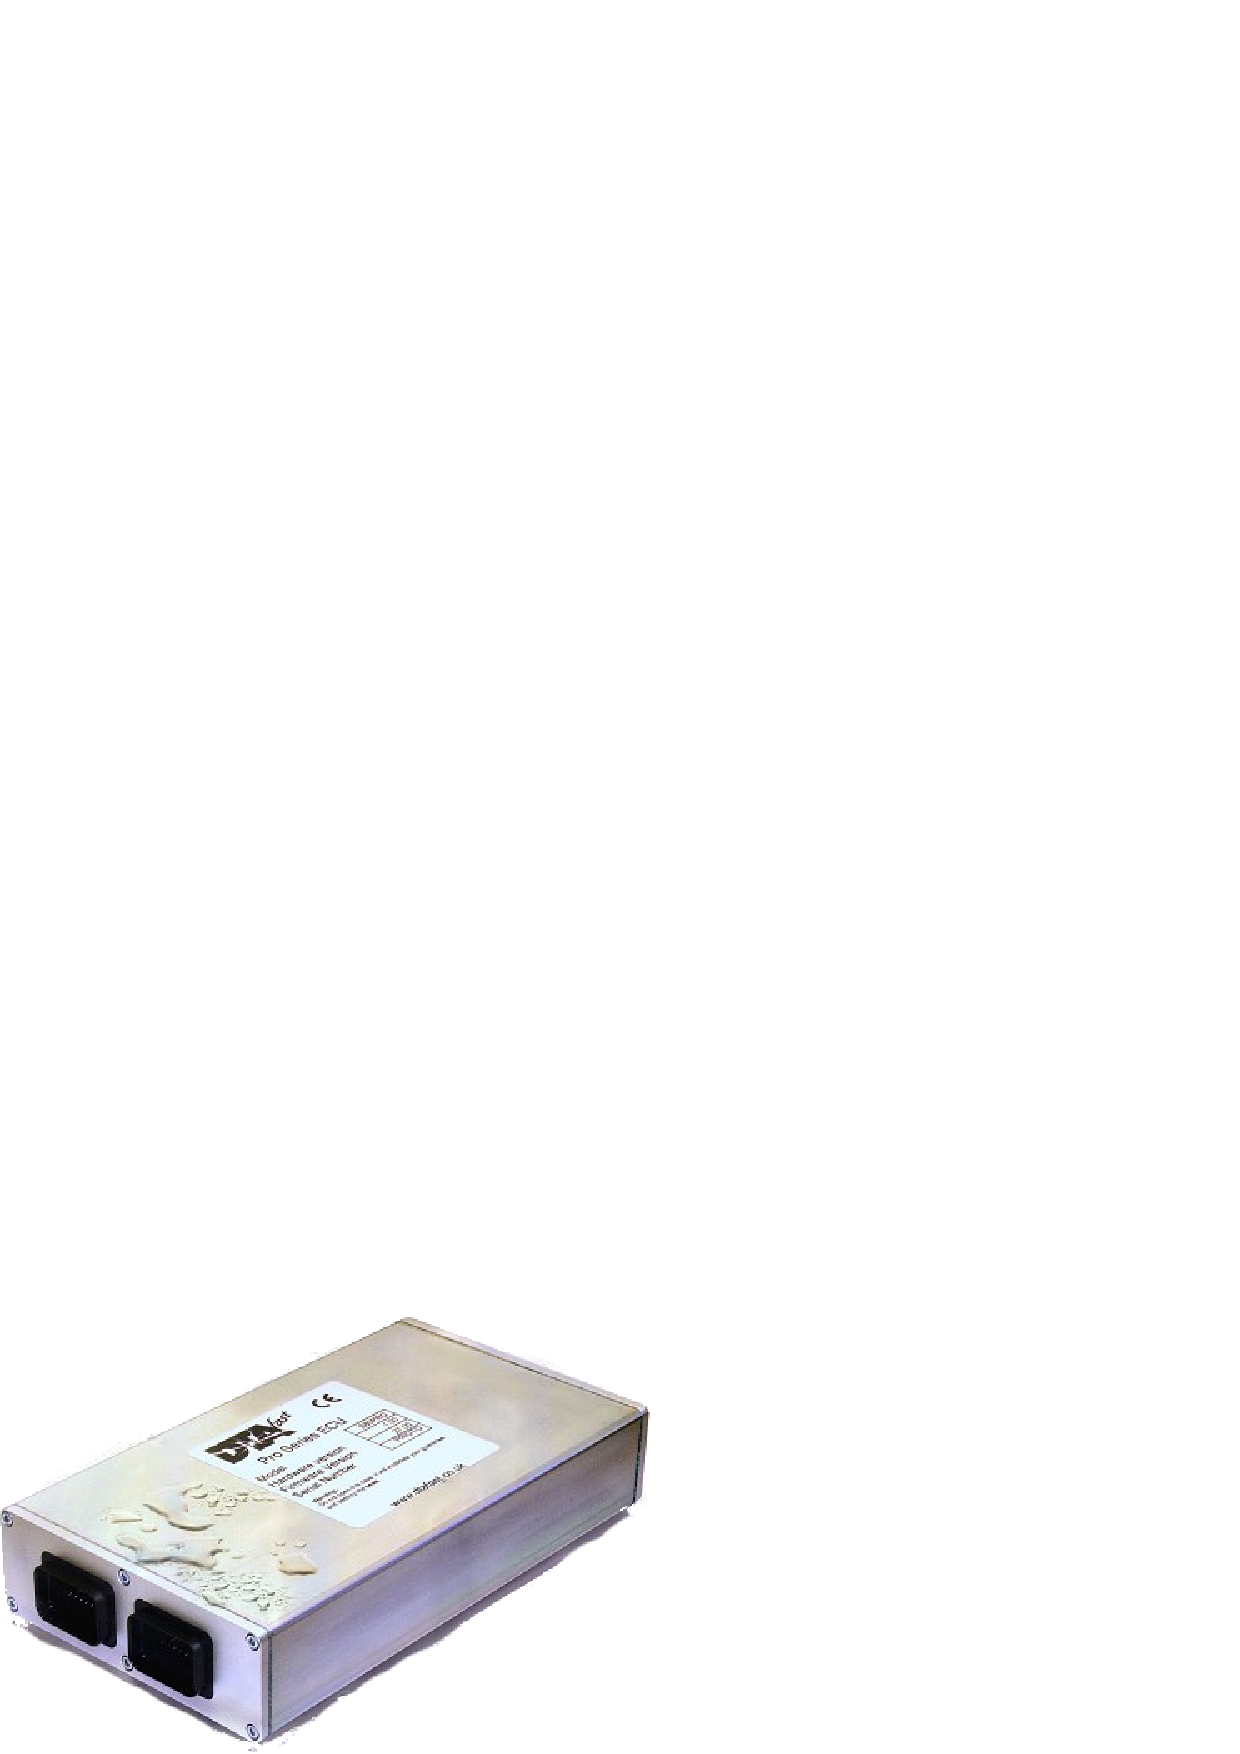
\includegraphics[scale=0.5]{Figures/s80.png}
\caption{The DTAFast S80Pro engine control unit.}
\label{fig:s80pro_product}
\end{figure}

\subsubsection{ECU Data interfaces\label{sec:background_ecu_data_interfaces}}

The ECU provides 3 digital communication methods:
\begin{itemize}
  \item An RS-232 link is used by the software that DTA provides for tuning and controlling the ECU. The serial protocol that the software uses is proprietary and undocumented.
  \item A read-only CAN bus interface that emits ECU data at a fixed frequency. The message format for the CAN data is documented in Appendix \ref{cha:ecu_can_spec}.
  \item Several CMOS-level discrete inputs:
  \begin{itemize}
    \item Launch Control toggle, which toggles the launch control feature in the ECU,
    \item Shift cut, which signals the ECU to reduce engine power before a downshift
    \item Traction control toggle, which toggles the traction control feature in the ECU,
    \item Traction control wet/dry, which switches between two different sets of traction control parameters in the ECU.
  \end{itemize}
\end{itemize}

Detailed descriptions of the ECU's launch control, shift cut, and traction control features can be found in the manual \cite{s80pro}.
 
\nomenclature{RS-232}{Recommended Standard 232, a byte-oriented serial communications protocol, typically asynchronous.}

\subsection{Intake and Exhaust}

Intake background, pressure waves, etc. Torque curve depends on length, 

\subsection{Research and Modelling of Variable Length Intake}

present research done by others on team, quantified runner length
dependence

intake length changes power

quantified length versus power on actual vehicle

chose optimal intake length

proposed variable length intake system for future work

\subsection{Starting System}

current requirements, starter motor, etc.


\section{Transmission}
\label{sec:background_transmission}

\subsection{Overview}

The Formula SAE 2010 vehicle uses a 6-speed manual sequential transmission to transmit power from the engine to the drive train. As in other types of manual transmissions, the sequential transmission works by engaging and disengaging several sets of gears with shift forks to obtain different gear ratios. A cast steel drum inside the transmission, called the \emph{shift drum}, has a series of complex grooves machined into it, in which the shift forks ride. Rotating the drum causes the forks to engage one gear and disengage the other. A ratcheting mechanism allows a single external lever, called the \emph{shift lever}, to rotate the drum forward and back by a discrete amount. Each full movement of the lever forwards or backwards causes a gear change up or down, respectively \cite{HowtoManualTransmission, cbr600}.

\subsection{Neutral Sensing}

The stock CBR600f4i engine is fitted with a simple 1-wire sensor which is connected to ground when the transmission is in neutral. The wire is left floating when the vehicle is in gear.

\subsection{Gear Position Sensing}

The stock transmission has no means of determining what gear the transmission is in; it can only determine when the transmission is in neutral using the aforementioned neutral sense wire. The ECU has provisions for reading a gear position potentiometer that can be attached to the shift drum, however this requires mechanical modification of the shift drum itself.

\subsection{Clutch}

The CBR600f4i is equipped with a multi-plate clutch which serves to transmit torque from the engine to the drivetrain. Layers of friction plates in the clutch are forced to rotate together when the clutch is engaged by a series of pre-tensioned springs. When the clutch is disengaged externally via the \emph{clutch lever}, the plates are separated and the drivetrain is allowed to spin freely from the engine. The clutch lever is actuated on the stock motorcycle with a hand lever via cable.

\subsubsection{Equations of Motion}

Equations of motion governing the clutch dynamics are:

\begin{equation}\label{eq:clutch_dynamics_a}
  J_c\dot{\omega}_c=T_c-T_d-b_c\cdot\left(\omega_c-\omega_t\right)
\end{equation}

\begin{equation}\label{eq:clutch_dynamics_b}
  \dot{T}_d=k\left(\phi_d\right)\cdot\left(\omega_c-\omega_t\right),
\end{equation}

where $J_c$ is the inertia of the clutch plates, $T_c$ the torque transmitted through the clutch, $b_c$ the clutch damping rate, and $\omega_c$ and $\omega_t$ are speeds of the clutch plates and transmission respectively \cite{clutch_control}.

A major point of interest in the operation of the clutch is the transition from fully disengaged to fully engaged, and vice-versa. In this state the clutch plates slip against each other as one rotates faster. \Citet{clutch_control} describe the torque transmitted through the clutch in slipping, $T_c{slip}$, as

\begin{equation}\label{eq:clutch_slip}
  T_c{slip}=F_n\mu R_a \cdot sgn\left(\omega_e-\omega_c\right),
\end{equation}

where $F_n$ is the normal force on the clutch plates, $\mu$ the coefficient of friction on the plate surfaces, and $R_a$ the radius of the plates, and $\omega_e$ and $\omega_c$ are the rotational velocities of the engine, and clutch discs, respectively. This shows that the amount of torque transmitted depends dynamically on the normal force $F_n$, which is proportional to the spring force pushing the plates together.

The second state of interested, as described by \cite{clutch_control}, is when the clutch is fully engaged and the plates are locked rotating at the same speed. The equation of motion for the engine, where the engine inertia $J_e$ is driven by the engine torque $T_e$ is given by:

\begin{equation}\label{eq:engine_motion}
  J_e\dot{\omega}_e=T_e-T_c.
\end{equation}

In the fully engaged state, $\omega_e=\omega_c=\omega$, a degree of freedom is removed, and by combining \eqref{eq:clutch_dynamics_a} and \eqref{eq:engine_motion} we obtain:

\begin{equation}
  \left(J_e+J_c\right)\dot{\omega}=T_e-Td-b_c\cdot\left(\omega\right),
\end{equation}

which shows that the system torque acts on the combined inertia of the plates as a single unit as the engine and transmission rotate at the same speed.

\subsubsection{Operation}

In normal operation of the car, the clutch is used in two specific cases\footnote{Use of the clutch is not required for upshifting, only a small reduction in engine torque.}:
\begin{enumerate}
  \item Accelerating the car from a stand-still, and
  \item Downshifting the transmission.
\end{enumerate}

When accelerating the car from a stand-still, two further sub-cases need to be considered: accelerating at the beginning of a race, or \emph{launching}, and moving the car forward in a slow, controlled, manner, which we have called \emph{crawling}. In launching the car, the goal is to gain as much momentum as possible by transmitting as much torque from the engine to the wheels as possible without breaking the tires loose. The goal of crawling the car is to accelerate slightly in a slow, completely controlled manner to under \unit{25}{\kilo\metre\per\hour}.

With purely manual clutch control (i.e., with a clutch lever), skillful completion of both of these operations requires a significant amount of skill on the part of the driver. To launch the car with minimal tire slip, the driver must modulate the throttle as well as the clutch position (allowing a certain amount of slip). Crawling a Formula SAE car is a similar operation, however due to the low torque output at low RPM of the engine, it is very easy to stall the engine by engaging the clutch too quickly. Additionally, it is often desirable to move the car slower than would be obtained by driving in first gear with the clutch fully engaged. This must be done by never fully engaging the clutch: the clutch state is alternated between slipping and fully disengaged.

Downshifting the transmission (changing from a higher gear to a lower gear) requires that the clutch be fully disengaged. In the fully manual operation, the driver must disengage the clutch, shift the transmission, blip the throttle\footnote{``Blipping'' the throttle is a short increase in throttle used to increase the engine RPM in order to match it closer to the clutch plate RPM}, and then re-engage the clutch. This is required since the torque transmitted by the clutch (Eq. \ref{eq:clutch_slip}) can be in the reverse direction, from the wheels to the engine.

\subsection{Previous Electropneumatic Implementation}

There are several disadvantages to a manually actuated transmission: it requires a great deal of dexterity and effort on behalf of the driver, shifting time is relatively slow (around \unit{1}{\second}) compared to an estimated theoretical minimum shift time ($<\unit{100}{\milli\second}$), and a mechanical linkage must be designed and packaged into the car.

For these reasons, Formula SAE vechicles have used electro-pneumatic actuation systems since 2008. This implementation replaced a purely mechanical clutch pedal and gear shifter with pneumatic actuators linked directly to the clutch and gear selector levers. Driver control was achieved with a set of electronic paddle switches located on the steering wheel: an up-shift paddle and a down-shift paddle. A compressed air cylinder is used to feed air to linear pneumatic actuators (cylinders), which apply force to the levers on the clutch and shift levers. Binary 3-way solenoid valves apply pressure to either side of the cylinders.

In 2007, electronic signalling of the solenoid valves was done with a set of switches on the steering wheel, which switched the low-current side of a set of relays. This in turn fed current to the solenoid valves. In this system, the timing of the mechanical interaction with the transmission was entirely dependent on how long the driver held down the paddles. This still required a lot of effort from the driver, and often resulted in missed shifts. It also caused heavy mechanical stress on the transmission as the actuators pressed hard on the shift levers.

The 2008/2009 Formula SAE car improved on the 2007 design by replacing the relays with high-current solid state drivers. The timing signals to the solenoid valves were precisely controlled with an ARM7 micro-controller. Shift timing could be programmed, and no longer depended on how long the paddles were held. This  reduced the effort required from the driver and also reduced possible driver error.

Although an improvement from previous years, several inherent drawbacks to the 2008/2009 shift system exist. The system uses a lot of air, and the air cylinder must be regularly refilled, which is a recurring expense.

The electropneumatic system relieves the driver from the burden of manually engaging the clutch. It also reduces shift-time by a factor of nearly ten. However, the system makes use of binary pneumatic valves which reduce the smoothness of the clutch engagement. The rate of engagement is limited by the air flow rate of the valve itself, resulting in a rough shifting sequence that is mechanically hard on the transmission. 

The most serious drawback of the system is that the position of the actuators was only binary (or trinary in the case of upshift/rest/downshift). It was only possible to engage or disengage the clutch at a constant rate, determined by the pressure in the system, the flow rate coefficient through the valves, and the diameter of the cylinder. Since launching the car requires careful modulation of the clutch position, which was not possible with a binary pneumatic system, launching the car still required a hand-lever.

Another limitation was posed by the lack of gear position sensing in the stock transmission. Although the system was able to determine when the transmission was in neutral, there was no way to determine if the gears had meshed after up- or down-shifting, and the signals sent to the actuator were therefore controlled open-loop with static timing tables.

\section{Braking}


\subsection{Overview}

Idea of braking and force distribution


\subsection{Mechanical Systems}


\subsubsection{Independant Hydraulic Systems}


\subsubsection{Balance Bar}


\subsection{Adjustment Difficulties}

Competition problems, manual adjustment difficulty, scope of adjustment,
tuneability lag

\section{Telemetry}

The Formula SAE 2010 vehicle utilizes several \emph{sensors} for monitoring key elements of the engine and drivetrain. As mentioned previously in Sec.\ \ref{sec:ECU}, the ECU uses these sensor readings to adjust the fuel injector and spark coil timings. However, the data gathered from these sensors can be very useful to determining the overall performance and health of the vehicle. 

Longitudinal and strain data are also important, as they can be used to track driver performance and to prevent mechanical fatigue and failure. Several sensors have been introduced in previous years to accomplish this, but the ECU makes no provisions for handling data that is not engine-related. A secondary device known as the \emph{Data Acquisition Device} (DAQ) \nomenclature{DAQ}{Data Acquisition Device} was introduced to record and broadcast secondary sensor data.

Both the ECU and the DAQ interface with proprietary software over hard-wired serial links. It was recognized in previous years that a wireless serial link would be required to gather data in real-time while the vehicle was actually performing in the field. Several solutions were introduced, including a \emph{cellular link} and a \emph{point-to-point XBee link}, but none of them have performed satisfactorily.

\subsection{Sensors}

The engine has a set of sensors attached to it that aide the ECU in determining the best parameters for controlling the fuel injection and spark coil timings. These include:

\begin{itemize}

\item The \emph{oxygen} sensor, which monitors the amount of oxygen present in the exhaust of the engine. This information, when coupled with other sensor information, can be used to calculate the air-fuel mixture ratio being combusted.

\item The \emph{Manifold Absolute Pressure} (MAP) sensor, which monitors the pressure in the manifold. The ECU uses this information to calculate the mass flow rate of air in the engine, which is also used to adjust the air-fuel mixture ratio being combusted.

\item The \emph{oil pressure} sensor, which is used to ensure enough oil pressure is present to keep the moving metal parts inside the engine are well-lubricated. A lack of oil pressure can cause an engine to \emph{seize}, meaning two moving parts in proximity have become stuck due to a lack of lubrication. This condition is typically fatal for an engine.

\item The \emph{water temperature} sensor, for monitoring the temperature of the coolant running through the engine block. The engine can become damaged if it is not adequately cooled, and an overheating engine can indicate to the crew that the coolant level is too low or there is a problem with the water pump.

\item The \emph{throttle position} sensor, to report the amount of throttle being applied by the driver, which in turn determines how much power is being demanded of the engine. This can be correlated with engine RPM data to determine how well the engine is responding to driver demands.

\item The \emph{cam position} sensor, which determines where the first cylinder is located in relation to its combustion cycle. This data is used to determine when to inject each cylinder with fuel to maximize power output.

\item The \emph{crank position} sensor, for determining the rotational speed of the crankshaft, which therefore measures the actual engine RPM. 

\end{itemize}

Motional and strain data are also important and require logging and analysis. Sensors to capture these data include:

\begin{itemize}

\item A \emph{Global Positioning System} (GPS), which is used to track the absolute geographic position of the vehicle. 

\item \emph{Accelerometers} and \emph{ground speed detectors}, that are attached to the vehicle to determine its acceleration and ground speed. Coupled with the GPS data, this can be used to measure driver performance and determine the best route to take through corners while on the track.

\item \emph{Strain gauges}, which are are attached to various members on the suspension and frame to determine the forces and strain the vehicle endures. These can be used to forecast fatigue and possible mechanical failure. 

\end{itemize}

\subsection{Data Acquisition Device (DAQ)}

The DAQ is required to convert the locational and strain sensor data into digital signals that can be transmitted to pit-crew laptops. The particular model of DAQ used is the DL1 from Race Technology. The DL1 is an expandable data logger with built-in \unit{20}{\hertz} GPS and 3-axis accelerometer \cite{DL1Dsheet}.

Race Technology provides a software suite that communicates with the DAQ using a documented serial protocol. Everything the DAQ logs is output over its serial channel in real-time.

\subsection{Cellular Link}

The 2005/2006 Formula team attempted to solve the wireless telemetry issue by using a CDMA-type cellular data link to broadcast ECU information to the pit crew. The team used a CDMA 1xRTT digital cellular network modem and a Soekris Engineering Linux-based microcomputer to interface between the ECU and cellular modem. The principle of operation was to broadcast ECU data through the modem to a local cell phone tower. The data would then be carried through the network, routed back to the local tower, and received by a modem connected to a laptop in the pit \cite{G26FinalRepo}.

This scheme created three prominent disadvantages:

\begin{itemize}

\item Expensive wireless data and roaming charges were incurred while the team competed in the United States. 

\item There was a massive amount of lag introduced as the data travelled through the American and Canadian cellular networks only to be received a few hundred metres away from the vehicle.

\item Only one device (the ECU) was able to be monitored in real-time. DAQ data had to be logged on the device itself and downloaded later.

\end{itemize}

\subsection{Point-to-Point XBee Link}

From 2007 onward, the Formula team utilized a pair of off-the-shelf 802.15.4/DSSS XBee Pro modems to wirelessly transmit information from the ECU to the pit crew. The XBee Pro modems established a transparent wireless link between the ECU and a pit-crew laptop. The ECU serial cable was plugged into a serial port located on a modem attached to the vehicle. An external antenna was run from the vehicle modem to the highest point of elevation on the vehicle, above the driver. The modem's twin was located in the pit, and attached to the pit crew laptop over another serial cable.

This scheme eliminated the need for a costly cellular solution and reduced transport lag, but was still far from optimal:

\begin{itemize}

\item Extensive interference was encountered, as similar modems on other competitor's vehicles were broadcasting on the same channel. When operating in "plug-and-play" mode, the broadcast channel must be adjusted manually on the device itself. Changing channels while in middle of a race is impossible, as it would require stopping the vehicle and exiting it.

\item As before, only the ECU data was being broadcast. To broadcast both ECU and DAQ data would require two modems, which was cost prohibitive.

\end{itemize}

\section{Driver Interface}

\subsection{Overview}

The driver interface consists of all the controls available to the driver to change the performance dynamics of the vehicle, all of the warning indicators that inform the driver of potentially hazardous situations, and all of the diagnostic information available to advise the driver on the overall condition of the vehicle.

An ideal driver interface is unobtrusive and requires as little driver attention and effort as possible. Controls required while the vehicle is in motion should be operable without the driver needing to divert their attention from the track. Warnings should be highly visible and discernible with minimal effort. Diagnostic information should not clutter or overwhelm the driver. Tuneable vehicle parameters should be presented to the pit crew with an intuitive interface that cannot be accidentally triggered by the driver.

\subsection{Transmission Control}

As discussed extensively in Sec. \ref{sec:background_transmission}, the driver must be able to up- and down-shift as quickly as possible. Early Formula SAE vehicles relied on a purely mechanical clutch and shift lever configuration. In 2008, the mechanical system was replaced with a pair of paddle shifters located on the steering wheel. Although the system being controlled by the paddles has evolved, the actual interface has remained constant for the past two incarnations.

The 2009 Formula SAE vehicle has feature known as \emph{neutral find}, which allows the driver to quickly shift the vehicle into neutral at the touch of a button. Normally, shifting into neutral would require the driver to down-shift until they reach neutral. This feature is especially useful for preventing the vehicle when leaving the track and entering the pit area. 

Another innovation of 2009 was the introduction of \emph{launch control}, which enabled the driver to accelerate rapidly from a stand-still without having to shift from neutral to first gear. The sensitivity of the engine means it is very easy to stall the motor if the clutch is engaged too quickly, especially when transitioning into first gear. Launch control eliminates this by monitoring the relative speeds of the engine and wheels, and modulates the clutch to provide the most power and traction to the wheels without stalling the engine. 
 
\subsection{Warning Indicators}

The driver must be alert to the possibility of the engine overheating, or of any drops in oil pressure that could cause damage to the engine. Previous implementations of the driver interface provided these warnings with simple LEDs that interfaced with the water temperature and oil pressure sensors. Although simple, the indicators were unreliable and would sometimes neglect to function, or would trigger when no problem was actually present. 

Several other warning indicators, such as a low voltage warning or an up-shift indicator, would be beneficial to the driver but have as of yet been out of scope for the Formula SAE team.

\subsection{Vehicle Diagnostics}

Diagnostic information about the vehicle, such as the state of the telemetry system, current gear, engine RPM, and so on have not been included in previous implementations. These diagnostics would be beneficial to the driver and the pit crew, but have been so far out of the scope of the previous implementations.




\chapter{Goals and Requirements\label{cha:goals}}

The guiding principle for the project is to incorporate changes that will improve the team's standing at competition. This can be achieved by improving the vehicle's performance, and by reducing the demand on the driver so that they may focus more on driving the vehicle. This chapter outlines the goals and requirements to which our design is built and measured against.

Each of the five major systems introduced in Ch. \ref{cha:background} have a set of goals and requirements associated with them. The limitations and shortcomings of each system that were encountered in previous years will be addressed. When possible, quantitative targets will be set based on research and recommendations from the mechanical engineers involved with the vehicle.

% \section{Engine}

The main goal of the engine system is to optimize the peak torque output of engine. This can be accomplished with a variable-length intake system, as suggested by Groening in \cite{LucasIntake}. Achieving this requires the ability to monitor the current engine speed and to mechanically adjust the runner lengths as needed.

\begin{itemize}
\item Automatically adjust the variable-length two-position intake to optimize peak torque output.
\item The intake runner length should be chosen automatically by determining the best position to optimize output power.
\item Changing the intake runner length positions should take no more than \unit{150}{\milli\second}.
\end{itemize}

\section{Transmission and Drivetrain\label{sec:goals_transmission}}

The overall goal for the transmission and drivetrain systems is to improve shift time and accuracy while reducing the effort required by the driver. To achieve this goal requires modifying and improving the existing electro-pneumatic system by improving both the pneumatics and the electronic transmission control system. 

\subsection{Shifting}

\begin{itemize}
\item Reduce the time to change gears to less than \unit{100}{\milli\second}. 
\item Implement a neutral-finding feature that will automatically downshift from the current gear to neutral in the shortest amount of time.
\item Implement an automatic up-shift feature that will up-shift the transmission without driver intervention to obtain the best possible acceleration.
\item Provide the ability to enable or disable the neutral-finding and automatic up-shifting features from the cockpit.
\end{itemize}

The average force required to actuate the shift lever on the CBR600f4i was measured using a fish scale to be \unit{5.42}{\newton\metre}. Any actuation method designed will need to be able to produce this torque, plus a factor of safety to account for wear and inconsistency.

\begin{itemize}
\item The shift lever actuator must be able to apply a minimum of \unit{6.00}{\newton\metre} of torque.
\end{itemize}

\subsection{Clutch Control}

\begin{itemize}
\item Completely automate all clutching operations, so that the driver never need modulate the clutch on their own.
\item Provide the ability to launch the car from a standstill by utilizing the ECU's launch control feature and engaging the clutch in such a way that prevents stalling and lurching.
\item Provide the ability to crawl the car from a standstill under \unit{25}{\kilo\metre\per\hour}, as well as be able to transition to regular driving, and back to a standstill without stalling or lurching.
\item Implement an anti-stall feature that protects the engine from stalling in the event of a spin-out by automatically shifting the transmission into neutral.
\item Provide the ability to enable or disable the launch, crawl, and anti-stall features from the cockpit.
\end{itemize}
  
The average force required to actuate the clutch lever on the CBR600f4i was measured using a torque wrench to be \unit{7.34}{\newton\metre}. Any actuation method designed will need to be able to produce this torque, plus a factor of safety to account for wear and inconsistency.

\begin{itemize}
\item The clutch lever actuator must be able to apply a minimum of \unit{8.00}{\newton\metre} of torque.
\end{itemize}  

\section{Braking}

The most desired improvement for the braking system is to eliminate the need for adjusting the brake bias manually, which requires substantial effort and time on behalf of the pit crew. Thus, the main goal for the braking system is to introduce an electronically-adjustable bias system. As the braking system is subject to mechanical wear and inconsistency, a secondary goal is to provide the ability to recalibrate the braking system at will.

\subsection{Bias Adjustment}

Eliminating the need to manually adjust the bias will improve the tunability of the vehicle. Allowing the driver to adjust the bias while on the track means the driver can adjust for varying track conditions like rain. This adjustment must occur quickly, because the driver may not apply the brakes during the adjustment.

\begin{itemize}

\item Allow the driver to adjust the brake bias from a control in the cockpit.
\item Provide a front-rear adjustment range of 30/70 to 70/30, with a resolution of $0.5\%$.
\item The bias must be able to be adjusted from one limit to the other in less than \unit{1}{\second}.
\item The bias must be adjustable while the vehicle is in motion.
\item The bias must not be adjusted while the brakes are being applied.

\end{itemize}

\subsection{Bias Calibration}

Because the system is subject to wear and inconsistency, the crew should be able to re-centre the balance bar as needed. This should be a short procedure, as there is usually not much time between events at a competition.

\begin{itemize}

\item Provide the ability to recalibrate the bias adjustment system to account for mechanical wear and inconsistency. 
\item It must take less than 30 seconds to complete the bias adjustment calibration.

\end{itemize}

\section{Telemetry\label{sec:goals_telemetry}}

The main goal of the telemetry system is to provide a reliable wireless connection between the two data-gathering devices on the vehicle (the ECU and DAC) and their respective software packages running on a pit crew laptop some distance away from the vehicle. 

\subsection{Engine Control Unit (ECU) \label{sec:goals_telemetry_ecu}}

The settings for the ECU link are fixed by the manufacturer, so our design must adapt to their demands. The software only operates with a serial link connected to the target computer, so the connection must be transparent to the software and the unit itself.

\begin{itemize}

\item Provide a wireless bi-directional serial link between the ECU software and module.
\item The link must operate at 57.6 KBps, 8 data bits, no parity bit, and 1 stop bit.
\item The link must be completely transparent to the software.

\end{itemize}

\subsection{Data Acquisition Unit (DAQ) \label{sec:goals_telemetry_dac}}

The settings for the DAQ link are not fixed by the manufacturer, but a minimum throughput is required to transmit all of the data being logged. Preliminary tests showed a baud rate of 38.4 KBps was satisfactory. Like the ECU, the software expects a serial link connected to the target computer, so the connection must also be transparent to the software and the DAQ.

\begin{itemize}

\item Provide a wireless uni-directional serial link between the DAQ software and module.
\item The link must operate at 38.4 KBps, 8 data bits, no parity bit, and 1 stop bit.
\item The link must be completely transparent to the software.
\item Provide a means of injecting data into the DAQ stream, such as engine RPM and other parameters, for monitoring by the DAQ software.
\item Provide a means of decoding the DAC stream on the vehicle itself to display information to the driver.

\end{itemize}

\subsection{Wireless Data Link \label{sec:goals_telemetry_range}}

The crew will be stationed in the pit area while the vehicle is engaged in its dynamic events at competition. The wireless link will need to be able to reach these laptops at all times. Most of the vehicles at competition will be using their own wireless telemetry systems. The possibility of interference requires a means of adjusting the broadcast channel while the vehicle is in motion. 

\begin{itemize}

\item Be able to interface with two laptops with a range of at least one kilometre.
\item Provide on-the-fly resolution of interference conflicts with other teams running similar wireless systems.
\item Indicate wireless signal strength to the driver and pit crew as a percentage with resolution of 10\% of maximum signal
strength. 

\end{itemize}

\section{Driver Interface}

The driver interface targets several major goals: providing access to critical features with a minimal amount of effort, providing visual feedback of the state of the vehicle without distracting the driver, and allowing the driver and pit crew to adjust the vehicle dynamic parameters as quickly and easily as possible. This is accomplished with the introduction of a driver display integrated into the steering wheel, and the ability to choose a set of vehicle parameters on the fly.

\subsection{Driver Controls}

Changing gears and accessing the automatic features of the transmission should be easy for the driver and require minimal effort. The driver also needs a means of actually starting the motor.

\begin{itemize}
\item Provide a means of shifting gears without manual timing or clutching.
\item Allow the driver to enable or disable all of the transmission features such as the auto up-shift feature, etc.
\item Provide the driver with a button to start or stop the engine. 
\end{itemize}

\subsection{Diagnostic Information}

The driver can maximize their performance when they are fully aware of the vehicle's state, and they can also avoid engine damage by knowing when it is reaching its operating limits. Diagnostic information can provide this to the driver, but it must be presented in a way that avoids distracting or overburdening the driver. Only critical features should have prominence on the display.

\begin{itemize}
\item Critical warnings regarding oil pressure and engine temperature must be delivered to the driver on an easy-to-read display.
\item The current gear and RPM should be displayed prominently on the screen so that they are readable at all times.
\item Supplementary vehicle performance information such as fuel level, oil pressure, and battery voltage should be made available to the driver without being a distraction.
\item The wireless telemetry link status should be displayed at all times.
\end{itemize}

\subsection{Vehicle Dynamic Adjustment}

Allowing the driver to adjust the electronically tuneable parameters of the vehicle on the fly means the driver can optimize performance of the vehicle for particular events at competition. Incorporating the ability to save the settings allows different drivers to setup the vehicle to their liking and dial-up the settings whenever they get behind the wheel.

\begin{itemize}
\item Provide an easy to use interface graphical interface to adjust vehicle dynamic parameters.
\item Allow the driver to choose between sets of dynamic vehicle parameters or `operating modes.'
\item Allow an operating mode to be selected with a single knob.
\item Disable adjustment of vehicle parameters above speeds of \unit{25}{\kilo\metre\per\hour}.
\item Allow the tuning of individual dynamic parameters and overwriting of preset operating modes.
\end{itemize}



\chapter{System Design\label{ch:design}}

\section{Architectural Overview}

Picture of the system overview.

Electropneumatic transmission actuators

Engine and transmission module

Braking module

Telemetry module

Driver control module

Located at points closest to the mechanical systems they interact
with.

Design systems as modularly as possible to reduce development time.

CAN Bus to reduce the number of point-to-point wiring required and
increase noise resiliancy, and interface with the existing ECU system
easily.

\section{Electro-Pneumatic System}

The electro-pneumatic system interfaces the engine and transmission module to the transmission's clutch and shift levers. The transmission controller portion of the engine and transmission module provide the control signals required to drive the electro-pneumatic system. The system design improves upon the previous generation discussed in Sec. \ref{sec:background_transmission} by targeting several of it's noted deficiencies while reusing aspects of the design that worked well.

A fully-electronic design was initially considered, but later abandoned. The finalized design calls for an improved valving scheme and a closed-loop feedback system. A thorough literature review was conducted to determine the best control system possible. 

The clutch actuation design incorporates a novel \emph{pulse-width modulation} (PWM) control scheme to allow for precise positioning control. The shift actuation design is unchanged from the previous implementation. 

\subsection{Fully-Electronic Consideration}

The possibility of using a fully electronic actuation system with geared DC motors was carefully considered. The control of such a system would be far simpler, as linear approximate models of DC motors are readily available. Reasonably priced gear-head motors from several suppliers were investigated. It was determined that any suitable fully-electronic system would be far heavier than it's pneumatic equivalent.

\subsection{Literature Review}

After deciding to keep a pneumatic actuation system, an improved valving scheme was proposed for the clutch, and sources of feedback were determined so that a closed-loop controller could be designed. Several academic papers were sourced that describe successful methods of pneumatic actuator control. \Citet{pneumatic_actuator} and \citet{adaptive_pneumatic} both use an electronically adjustable proportioning valve and a dual-acting cylinder. Proportioning valves are expensive (approximately \$300 from local suppliers) in comparison with binary solenoid valves (under \$50.)

Another approach by \citet{accurate_position} uses PWM signalled 3-way solenoid valves to control the air in and out of both sides of a dual-acting cylinder. By varying the duty cycle of the input signals, they were able to modulate the effective mass air flow rate through the cylinder ports: with the valve open, air would tend to flow from the high-pressure source into the cylinder, and with the valve closed, air would flow from the pressurized cylinder out through the exhaust port of the valve. This valving scheme allowed for a high degree of positional accuracy, however a large amount of air would be consumed during operation, as air is constantly being exhausted.

The dimensions of the pneumatic cylinders used in any implementation of this design are the same as those used in the previous designs. For this reason they will not be specified here.

\subsection{Mechanical Components}

A diagram of the mechanical portion of the pneumatics system is shown in Fig. \ref{fig:pneumatics_design}. As in the previous design, an on-board compressed air tank is fitted with a pressure regulator, which regulates the system pressure to approximately $\unit{0.8}{\mega\pascal}$. Four solenoid valves controlled with signals $U_U$, $U_D$, $U_A$, and $U_B$ control the flow of air to and from 2 pneumatic actuators.

\begin{figure}[H]
	\centering
	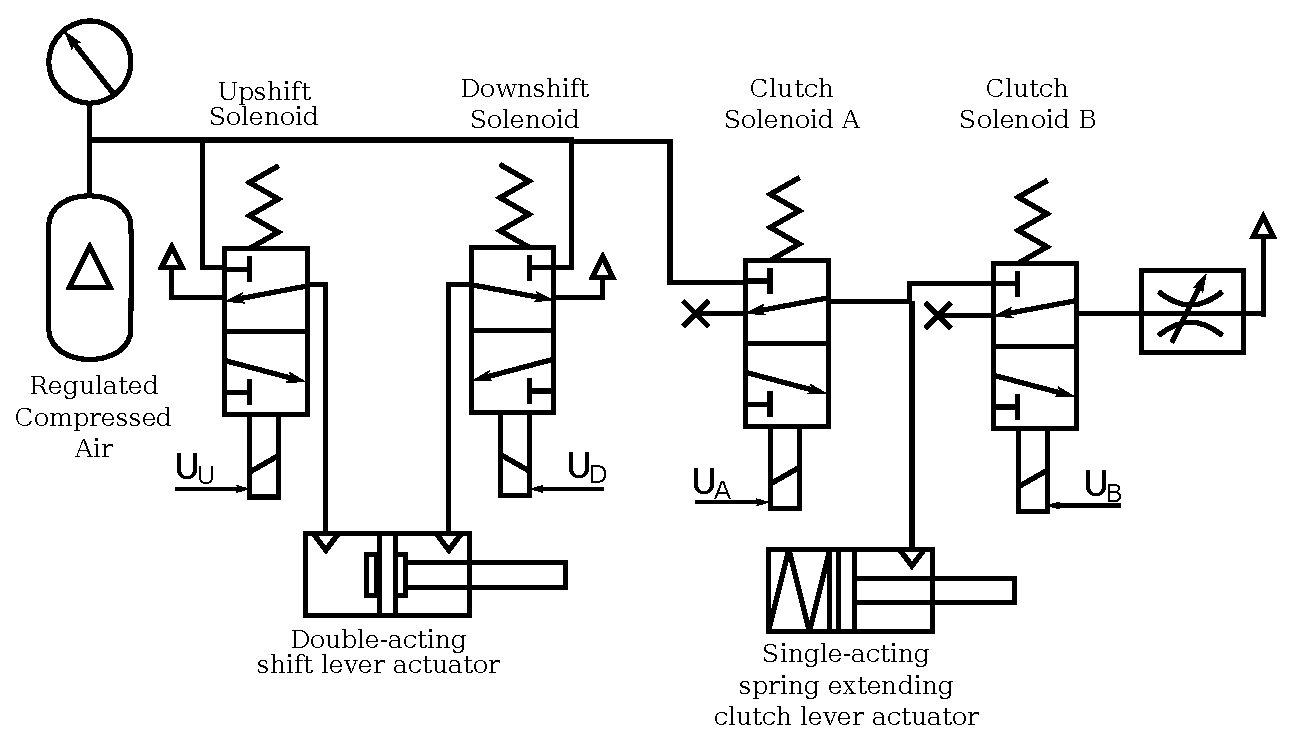
\includegraphics[scale=0.5]{design/figures/pneumatics}
	\caption{Transmission control pneumatics design.}
	\label{fig:pneumatics_design}
\end{figure}

\subsection{Clutch Lever Actuation}
\nomenclature{PWM}{Pulse Width Modulation}
\nomenclature{$U_U$, $U_D$}{Output signals from the transmission controller to the upshift and downshift solenoids.}
\nomenclature{$U_A$, $U_B$}{Pulse width modulated output signals from the transmission controller to clutch solenoids A and B.}

The three approaches described in \cite{pneumatic_actuator, adaptive_pneumatic, accurate_position} considered the possibility of a highly dynamic load on the actuator. The load seen by the clutch actuator is far more predictable than the loads they expected and is only uni-directional. Since the vehicle is only equipped with a limited supply of air, conservation is a concern. Taking these factors into account, a single-acting cylinder with a return spring is specified for the clutch, and we propose a new valving scheme that allows a degree of controllability over the actuator while conserving as much air as possible.

The cylinder visible on the right of Fig. \ref{fig:pneumatics_design}, actuates the clutch lever. Precise control of the clutch is accomplished with fast solenoid valves \emph{Clutch Solenoid A} and \emph{Clutch Solenoid B}. These valves are signalled with \emph{pulse width modulated} (PWM) signals, which modulate the average mass air flow rate into and out separately of the cylinder. Positional feedback for the clutch cylinder is provided by a combination of an internal magnet on the piston in the cylinder and a magnetic sensing membrane potentiometer.

Both clutch solenoids are shown as 3-way (with exhaust ports) valves in Fig. \ref{fig:pneumatics_design}, but the valves are used in a 2-way configuration with the exhaust ports plugged.  This results in the following operation:

\begin{enumerate}
  \item When the pulse width modulated control signal $U_A$ to Clutch Solenoid A is non-zero, the valve will open, and air will flow into the cylinder at a rate proportional to the duty cycle, disengaging the clutch.
  \item When pulses no longer arrive at Clutch Solenoid A (or the duty cycle of $U_A$ approaches 0), the valve remains closed, and any air in the cylinder is trapped. The clutch maintains is position.
  \item When the pulse width modulated control signal $U_B$ to Clutch Solenoid B is non-zero, the valve will open, and any pressure differential between the cylinder and atmosphere will cause air to flow out of the cylinder to atmosphere at a rate proportional to the duty cycle. The clutch springs and the cylinders' internal spring work to return the actuator position to rest, and the clutch engages.
\end{enumerate}

An additional adjustable flow rate control valve (visible on the far right in Fig. \ref{fig:pneumatics_design}) was added to the design to allow additional tuning for during clutch engagement. The electro-pneumatic actuation system meets the controllability requirements outlined in \ref{sec:goals_transmission} when coupled with the transmission controller on the engine and transmission module. No air is wasted in disengaging the clutch and holding the position because the fill and exhaust operations are separately controlled with two valves.

\subsection{Shift Lever Actuation}

The shift lever does not require the same level of control as the clutch, and as such the design of the valving has not changed over previous implementations. Two binary valves are used with a dual-acting cylinder. The first actuator (visible on the left of Fig. \ref{fig:pneumatics_design}) actuates the shift lever between 3 different positions: up-shift, down-shift, and rest-state. The transmission spring-loads the lever to automatically return to the rest-state, which is half-way through the actuator stroke. Applying pressure to one port will pull the lever up, and applying pressure to the other port will pull the lever down.

Current gear position is determined with a potentiometer that is mechanically linked to the shift drum. Control and timing are generated by the engine and transmission controller.


\section{Engine and Transmission Module}

The engine and transmission module provides optimized selection of the variable-length intake, changes gears at the driver's request without requiring manual clutching, and provides transmission features that make driving easier. Figure \ref{fig:design_engine_overview_block} shows an overview of the engine and transmission module and it's interactions with the environment.

\begin{figure}[H]
	\centering
 	\begin{tikzpicture}[auto, node distance=2cm, draw=black!70, >=stealth', font=\footnotesize]
  \node [block, blue shiny, minimum width=4cm, text width=4cm, right=-1cm, node distance=1.5cm] (module) {Engine and\\Transmission Module};

  \node at ($(module.east)+(1cm,0)$) [block, text width=0.8cm] (ecu) {ECU};

  \node [bus, above of=module, node distance=1cm] (bus1) {};
  \node [bus, above of=ecu, node distance=1cm] (bus2) {};

  \draw [<->, thick] (ecu) to (module);

  \draw [-, line width=3pt] (bus1) --  ++(-1cm,0);
  \draw [-, line width=3pt] (bus1) -- node[label=above:CAN Bus]{} (bus2) -- ++(1cm, 0);
  \draw [<->, thick] (module) -- (bus1);
  \draw [<->, thick] (ecu) -- (bus2);

  \node at ($(module.west)!0.5!(module.south)+(0,-1.25cm)$) [red shiny, circle, label={[text width=1.5cm, rotate=90, below=5pt, left=10pt]below right:Servo}] (motor) {M};
  \node [block, left of=motor, node distance=1.5cm, text width=1cm] (intake) {Intake};

  \draw [<-, thick] (intake) -- (motor);
  \draw [<-, thick] (motor) -- ($(module.south west)!(motor.north)!(module.south)$);

  \node [block, below of=module, inner xsep=0pt, right=0cm, node distance=1.5cm] (pneumatics) {Electro-Pneumatic system};
  \draw [<-, thick] (pneumatics) -- ($(module.south west)!(pneumatics.north)!(module.south)$);

  \node [block, right of=pneumatics, text width=2cm, node distance=3cm, above=0.25cm] (shift) {Shift Lever};
  \node [block, right of=pneumatics, text width=2cm, node distance=3cm, below=0.25cm] (clutch) {Clutch Lever};

  \draw [<-, thick, dashed] (clutch) -- ($(pneumatics.north east)!(clutch.west)!(pneumatics.south east)$);
  \draw [<-, thick, dashed] (shift) -- ($(pneumatics.north east)!(shift.west)!(pneumatics.south east)$);

  %%% Legend

  \draw [->, thick] ($(shift.east)+(2cm,0cm)$) -- ++(0.5cm,0) node [label={[font=\tiny]below:Electrical}] {} -- ++(0.5cm,0);
  \draw [->, thick, dashed] ($(clutch.east)+(2cm,0cm)$) -- ++(0.5cm,0) node [label={[font=\tiny]below:Mechanical}] {} -- ++ (0.5cm,0);
\end{tikzpicture}

	\caption{An overview of the engine and transmission module and it's environmental interactions.}
	\label{fig:design_engine_overview_block}
\end{figure}

The intake runner position is mechanically actuated with a \emph{servo motor}. The module generates the control signals required by electro-pneumatic system to actuate both the clutch and shift levers. The ECU interfaces with the module both directly through discrete inputs and through the CAN bus.

\subsection{Driver-Initiated Processes}

The major processes of the engine and transmission module are \emph{up-shifting}, \emph{down-shifting}, and \emph{neutral find}. They are described at a high level using flow charts. Requests to perform these processes are broadcast over the network from the driver interface. The module listens for these requests and executes the correct process accordingly.

\subsubsection{Up-Shifting}

The up-shift procedure is illustrated in \ref{fig:transmission_upshift_flow}. Up-shifting does not require disengaging the clutch, merely a small decrease in engine RPM. The ECU provides a shift-cut feature to cut spark to the engine during a shift operation to avoid the driver having to manually modulate the throttle during a shift.

\begin{figure}[H]
	\centering
	\begin{tikzpicture}[auto, node distance=2cm, draw=black!70, >=stealth', font=\scriptsize]
  \node[start, text width=1.2cm] (start) {Upshift Request};
  \node [decision, right of=start, text width=1cm, inner sep=0pt, node distance=2.5cm] (at_top) {Top\\gear?};
  \node [end, below of=at_top] (done) {Done};
  \node [block, right of=at_top, text width=1.5cm, node distance=2.5cm] (shiftcut) {Enable shiftcut};

  \node [block, right of=shiftcut, text width=1.5cm, node distance=2.5cm] (wait_shiftcut) {Wait for RPM drop below $RPM^{TH}_{cut}$};
  \node [block, right of=wait_shiftcut, text width=1.5cm, node distance=2.5cm] (upshift) {Engage upshift solenoid};
  \node [block, right of=upshift, text width=1.5cm, node distance=2.5cm] (wait_upshift) {Wait for shift feedback};
  \node [block, below of=wait_upshift, text width=1.5cm] (upshift_off) {Disengage upshift solenoid};
  \node [block, left of=upshift_off, text width=1.5cm, node distance=2.5cm] (shiftcut_off) {Disable shiftcut};

  \draw [->, thick] (start) -- (at_top);
  \draw [->, thick] (at_top) -- node[]{yes} (done);
  \draw [->, thick] (at_top) -- node[]{no} (shiftcut);

  \draw [->, thick] (shiftcut) -- (wait_shiftcut);
  \draw [->, thick] (wait_shiftcut) -- (upshift);
  \draw [->, thick] (upshift) -- (wait_upshift);
  \draw [->, thick] (wait_upshift) -- (upshift_off);
  \draw [->, thick] (upshift_off) -- (shiftcut_off);
  \draw [->, thick] (shiftcut_off) -- (done);
\end{tikzpicture}

	\caption{The transmission up-shift procedure.}
	\label{fig:transmission_upshift_flow}
\end{figure}

The up-shift process depends upon engine RPM and gear position, both of which are provided by the ECU. The shift-cut feature is engaged on the ECU to drop the engine RPM by a small amount known as the cut RPM threshold, or $RPM^{TH}_{cut}$. The exact value of $RPM^{TH}_{cut}$ can be tuned on the ECU. Once the RPM reaches the cut threshold, the upshift solenoid is engaged, which actuates the pneumatics to push the shift lever. Once the module receives notification that the current gear has incremented, the pneumatics are relaxed, and shift cut feature is disengaged.

\nomenclature{$RPM^{TH}_{cut}$}{The threshold RPM is expected to drop when shift-cut is engaged for no-lift up-shifting.}

\subsubsection{Down-Shifting}

The down-shift procedure is illustrated in \ref{fig:transmission_downshift_flow}. The downshift procedure differs from the upshift procedure in that the downshift requires use of the clutch. 

\begin{figure}[H]
	\centering
	\begin{tikzpicture}[auto, node distance=2cm, draw=black!70, >=stealth', font=\scriptsize]
  \node[start, text width=1.4cm] (start) {Downshift Request};
  \node [decision, right of=start, text width=1cm, inner sep=0pt, node distance=2.5cm] (in_neutral) {In neutral?};
  \node [end, below of=in_neutral] (done) {Done};
  \node [block, right of=in_neutral, text width=1.5cm, node distance=2.5cm] (clutchin) {Disengage clutch};

  \node [block, right of=clutchin, text width=1.5cm, node distance=2.5cm] (downshift) {Engage downshift solenoid};
  \node [block, right of=downshift, text width=1.5cm, node distance=2.5cm] (wait_downshift) {Wait for shift feedback};
  \node [block, right of=wait_downshift, text width=1.5cm, node distance=2.5cm] (downshift_off) {Disengage downshift solenoid};
  \node [block, below of=downshift_off, text width=1.5cm] (wait_clutchin) {Wait for clutch-in request};
  \node [block, left of=wait_clutchin, text width=1.5cm, node distance=2.5cm] (clutchout) {Engage clutch};

  \draw [->, thick] (start) -- (in_neutral);
  \draw [->, thick] (in_neutral) -- node[]{yes} (done);
  \draw [->, thick] (in_neutral) -- node[]{no} (clutchin);

  \draw [->, thick] (clutchin) -- (downshift);
  \draw [->, thick] (downshift) -- (wait_downshift);
  \draw [->, thick] (wait_downshift) -- (downshift_off);
  \draw [->, thick] (downshift_off) -- (wait_clutchin);
  \draw [->, thick] (wait_clutchin) -- (clutchout);

  \draw [->, thick] (clutchout) -- (done);
\end{tikzpicture}

	\caption{The transmission down-shift procedure.}
	\label{fig:transmission_downshift_flow}
\end{figure}

From the drivers perspective, down-shifting is a two-stage process:

\begin{enumerate}
  \item The driver pulls and holds the down-shift paddle on the steering wheel to request the gear change; and
  \item The driver releases the down-shift paddle to requests the clutch re-engage.
\end{enumerate}

Adding this extra clutch engagement request allows the driver to delay re-engagement of the clutch so that they can blip the throttle to avoid engine compression and the possibility of a spinout when the clutch plates re-engage\footnote{"Blipping" was previously described in Sec. \ref{sec:background_transmission}.}. 

Once the driver requests a down-shift, the clutch is disengaged and the down-shift solenoid is engaged to change gears. Once the correct gear has engaged, the solenoid is disengaged and the controller waits for the driver to release the down-shift paddle. When the paddle is released, the clutch is re-engaged. A minimum clutch disengagement time $t_{clutch_{min}}$ is observed in the event the driver pulls the paddle and releases it without any delay. This parameter is tunable.

\nomenclature{$t^{clutch}_{min}$}{Minimum clutch disengagement time during a downshift request.}

\subsubsection{Neutral Find}

Neutral find can be used by the driver to quickly shift into neutral when entering the pit area, without having to manually cycle through gears. The procedure is illustrated in \ref{fig:transmission_neutralfind_flow}.

\begin{figure}[H]
	\centering
	\begin{tikzpicture}[auto, node distance=2cm, draw=black!70, >=stealth', font=\scriptsize]
  \node[start, text width=1.4cm] (start) {Start};
  \node [decision, right of=start, text width=1.2cm, inner sep=0pt, node distance=2.5cm] (in_neutral1) {Neutral?};
  \node [end, below of=start, node distance=1.5cm] (done) {Done};
  \node [block, right of=in_neutral1, text width=1.5cm, node distance=2.5cm] (clutchin) {Disengage clutch};
  \node [block, right of=clutchin, text width=1.5cm, node distance=2.5cm] (downshift) {Downshift};
  \node [decision, right of=downshift, text width=1.2cm, inner sep=0pt, node distance=2.5cm] (in_neutral2) {Neutral?};

  \node [block, below of=clutchin, text width=1.5cm, node distance=1.5cm] (clutchout) {Engage clutch};

  \draw [->, thick] (in_neutral1.south) -- node[]{yes} (in_neutral1.south |- clutchout);

  \draw [->, thick] (start) -- (in_neutral1);
  \draw [->, thick] (in_neutral1) -- node[]{no} (clutchin);
  \draw [->, thick] (clutchin) -- node[coordinate](x1){} (downshift);
  \draw [->, thick] (downshift) -- (in_neutral2);
  \draw [->, thick] (in_neutral2.north) -- node[above=3pt]{no} ++(0,0.25cm) -| (x1);

  \draw [->, thick] (in_neutral2.south) |- node[]{yes} (clutchout);
  \draw [->, thick] (clutchout) -- (done);
\end{tikzpicture}

	\caption{The transmission neutral find procedure.}
	\label{fig:transmission_neutralfind_flow}
\end{figure}

When the driver engages the neutral find feature, the transmission controller disengages the clutch and downshifts until the neutral sensor indicates the transmission has reached the neutral gear. The clutch lever is then released with the transmission in neutral. If the driver attempts to engage the feature while the vehicle is already in neutral, the procedure is aborted.

\subsection{Variable Intake}

The length of the intake runners is modulated automatically to provide the optimal torque output for the current engine RPM. The control flow chart is shown in Fig. \ref{fig:engine_varintake_flow}. 
\begin{figure}[H]
	\centering
	\begin{tikzpicture}[auto, node distance=2cm, draw=black!70, >=stealth', font=\scriptsize]
  \node [start, text width=1.4cm] (start) {Start};
  \node [block, right of=start, text width=1.5cm, node distance=2.5cm] (update) {Update RPM};
  \node [decision, right of=update, text width=1cm, inner sep=0pt, node distance=2.5cm] (ideal) {Ideal length?};

  \node [block, right of=ideal, text width=1.5cm, node distance=2.5cm] (switch) {Switch lengths};
  \node [block, right of=switch, text width=1.5cm, node distance=2.5cm] (wait) {Wait for lockout};

  \draw [->, thick] (start) -- (update);
  \draw [->, thick] (update) -- (ideal);
  \draw [->, thick] (ideal) -- node[above]{no} (switch);
  \draw [->, thick] (switch) -- (wait);
  \draw [->, thick] (wait) -- ++(0, -1.5cm) node[coordinate](x1){} -| ($(start.east)!0.5!(update.west)$);
  \draw [->, thick] (ideal) -- node[]{yes} (ideal.south |- x1);

\end{tikzpicture}
	\caption{The variable intake adjustment flow.}
	\label{fig:engine_varintake_flow}
\end{figure}

Optimizing the runner length requires coordination with the ECU to acquire the latest RPM values. A set-point RPM value to be determined will act as a cross-over point at which the runner length changes. As the engine RPM crosses over this line, the runner length is modulated. A brief timeout period exists to prevent the runner length from oscillating if the driver is operating near the cross-over point.

\subsection{Advanced Transmission Features}

The transmission portion of the module implements several features to aide the driver. The driver can enable or disable these features from the driver interface. The module will listen for feature requests over the network and act accordingly.

\subsubsection{Auto Up-shift}

This feature of the engine module is aimed primarily at improving performance in the acceleration event. Based on known torque curves, a table of optimal shift points in the RPM range is developed. As the engine reaches the top RPM for a given gear, the engine module will automatically upshift to the next gear, without any driver input. All the driver needs to do is maintain full throttle, and hang on.

\subsubsection{Launch}

Full-throttle launch uses an important feature of the ECU called launch control. From a stand-still, the slip ratio of the driven wheels to the non-driven wheels is monitored, and the engine output power is reduced until the ratio reaches 1:1. Drivers use this feature by maintaining full-throttle at the starting line while holding the brake pedal. As soon as the brake pedal is released, the the engine module will release the clutch in a controlled manner in an attempt to get the best possible acceleration.

\subsubsection{Crawl}

Part-throttle launch is a feature designed to mimic an automatic transmission. By controlling the clutch position, and thereby modulating the amount of torque transferred to the wheels for a short period of time, the car can be made to creep slowly from a stand-still. This will be used when driving up to the starting line of various dynamic events.

\subsection{Hardware}

A high-level overview of the module's hardware design is shown in figure \ref{fig:engine_hardware_design_block}. The module makes use of a \emph{micro-controller} to execute all of the controller software. 

\vspace{1em}
\begin{figure}[H]
	\centering
	\begin{tikzpicture}[auto, node distance=2cm, draw=black!70, >=stealth']

  \node [block, font=\scriptsize, text width=1.5cm, inner xsep=0, minimum height=1cm] (intake) {Intake};
  \node [red shiny, circle, below of=intake, node distance=1.15cm, inner sep=1pt, label=right:Servo] (servo) {M};

  \draw [->, dashed, thick] (servo) -- (intake);

  %%% Balance bar and EOT switches
  \node [block, right of=intake, font=\scriptsize, text width=1.5cm, node distance=3cm, inner xsep=0, minimum height=1cm] (clutch) {Clutch Actuator};
  \node [block, right of=clutch, font=\scriptsize, text width=1.35cm, inner xsep=0, minimum height=1cm] (clutch_solenoids) {Clutch Solenoids};
  \node [block, right of=clutch_solenoids, font=\scriptsize, text width=1.35cm, inner xsep=0, minimum height=1cm] (shift_solenoids) {Shift Solenoids};
  \node [block, right of=shift_solenoids, font=\scriptsize, text width=1.5cm, inner xsep=0, minimum height=1cm] (shifter) {Shift Actuator};

  \node at ($(clutch_solenoids)!0.5!(shift_solenoids)+(0,-2cm)$)
    [block, node distance=1cm, text width=2.5cm, font=\scriptsize, minimum width=3cm] (driver) {Solenoid Drivers};

  \node [block, right of=shifter, font=\scriptsize, text width=1.5cm, inner xsep=0, minimum height=1cm, node distance=3cm] (ecu) {ECU};

  \draw [<-, thick] (clutch_solenoids) -- ($(driver.north west)!(clutch_solenoids.south)!(driver.north east)$);
  \draw [<-, thick] (shift_solenoids) -- ($(driver.north west)!(shift_solenoids.south)!(driver.north east)$);
  \draw [->, dashed, thick] (clutch_solenoids) to (clutch);
  \draw [->, dashed, thick] (shift_solenoids) to (shifter);

  \draw [->, thick] (shifter) to (ecu);

  \node [block, below of=clutch, text width=1.5cm] (adc) {ADC};
  \draw [->, thick] (clutch) to (adc);

  %%% Microcontroller block
  \path ($(intake.south west |- adc.south west) + (0,-1cm)$) node (mu1) {};
  \path ($(shifter.south east |- driver.south east) + (0,-1cm)$) node (mu2) {};

  \node [block, fit=(mu1) (mu2), inner xsep=0, minimum height=1cm] (micro) {Microcontroller};

   \draw [<-, thick] (servo.south) -- ($(micro.north west)!(servo.south)!(micro.north east)$);
   \draw [->, thick] (adc.south) -- ($(micro.north west)!(adc.south)!(micro.north east)$);
   \draw [<-, thick] (driver.south) -- ($(micro.north west)!(driver.south)!(micro.north east)$);

% 
%   \draw [->, thick] (eot1.south) -- ($(micro.north west)!(eot1.south)!(micro.north east)$);
%   \draw [->, thick] (eot2.south) -- ($(micro.north west)!(eot2.south)!(micro.north east)$);
% 
%   \draw [<-, thick] (driver.south) -- ($(micro.north west)!(driver.south)!(micro.north east)$);

  \draw [<-, thick] (ecu.south) |- ($(shifter.south) + (0,-0.5cm)$) node[name=t]{} -- ($(micro.north west)!(t)!(micro.north east)$);

  %%% CAN Bus

  \node at ($(micro.east)+(1.5cm,0)$) [block, name=can, inner xsep=2pt] {CAN Transceiver};
  \draw [<->, thick] (micro) to (can);
  \draw [-, line width=3pt] (ecu.east) -- ++(0.5cm,0) |- node[name=can1,coordinate,label={[rotate=90]below:CAN Bus}]{} (can);
  \draw [-, line width=3pt] (can1) -- ++(0,-1cm);

  %%% Background

   \begin{pgfonlayer}{background}
     \path (intake.south west |- adc.north west)+(-0.3,0.3) node (a) {};
     \path (can.south east)+(+0.2,-0.2) node (b) {};
     \path[module] (a) rectangle (b);
   \end{pgfonlayer}

  %%% Legend

  \draw [->, thick] ($(micro.south west)+(0.5cm,-0.5cm)$) -- ++(0.5cm,0) node [label={[font=\tiny]below:Electrical}] {} -- ++(0.5cm,0);
  \draw [->, thick, dashed] ($(micro.south west)+(2cm,-0.5cm)$) -- ++(0.5cm,0) node [label={[font=\tiny]below:Mechanical}] {} -- ++ (0.5cm,0);
\end{tikzpicture}

	\caption{A block diagram of the engine and transmission module hardware.}
	\label{fig:engine_hardware_design_block}
\end{figure}

\nomenclature{ADC}{Analog-to-Digital Converter}
\nomenclature{GPIO}{General Purpose Input-Output}

Inter-module communication over the CAN bus is mediated with a \emph{CAN transceiver}. An \emph{analog-to-digital converter} (ADC) samples the position of the clutch. Unique to the module are high-current \emph{solenoid driver} that are used to engage the solenoid valves that actuate the clutch and shift levers. Discrete signals to the ECU are connected to \emph{general purpose input-output} (GPIO) lines of the micro-controller.

\subsubsection{Micro-controller}

\nomenclature{EEPROM}{Electronically-Erasable Programmable Read-Only Memory}

The main purpose of the micro-controller is to execute system control software. The micro-controller should be in-circuit programmable and debuggable to speed development, with a built-in CAN controller. It should also have built-in \emph{electronically-erasable programmable read-only memory} (EEPROM) for holding configuration parameters.

\subsubsection{CAN Transceiver}

The CAN transceiver translates the digital bits generated by the CAN controller into a differential line-coded signal suitable for broadcasting over the bus. Both ends of a CAN bus must be terminated with a \unit{120}{\ohm} resistor \cite{MCP2551}. The module should be configurable to terminate the bus if desired.

\subsubsection{Analogue-to-Digital Converters}

The analogue-to-digital converters sample the clutch position sensor. The output voltage of the particular sensor used is \unit{0-5}{\volt}, corresponding to 0-100\% engagement of the clutch. The required sampling frequency is \unit{1}{\kilo\hertz}.

\subsubsection{Solenoid Drivers}

High-current solenoid drivers provide current to the solenoids that actuate the clutch and shift levers. The actual amount of current required depends on the particular implementation. We must use drivers that can source enough current to provide the torque required to actuate the clutch and shift levers. 
 
\subsubsection{ECU Control Signals}

The engine and transmission module have several outputs to control pins on the ECU:

\begin{itemize}
  \item the launch control pin, which enables and disables the launch control feature;
  \item the shift cut pin, which, when held high, enables shift cut;
  \item the traction cut percent pin, which is a \unit{0-5}{\volt} analog input that sets the amount of wheel slip threshold for traction control;
  \item the traction control on/off pin, which toggles the traction control feature; and
  \item the traction control wet/dry pin, which swaps between two traction control presets.
\end{itemize}

\subsection{Software}

A block-diagram overview of the software design is shown in Fig. \ref{fig:engine_software_design_block}. The functionality of the system is separated into an \emph{intake manager} and a \emph{transmission manager}. The managers interact with a set of \emph{hardware abstraction interfaces} to perform their tasks. A \emph{PWM generator} provides the signals required to interact with the electro-pneumatic system. The entire process is overseen by a \emph{module coordinator}.

\begin{figure}[H]
	\centering
%	\tikzstyle{big arrow} = [>=latex, line width=4pt, gray]

\begin{tikzpicture}[auto, node distance=2cm, draw=black!70, >=stealth', font=\scriptsize]
  %\draw[help lines] (-1,-5) grid (8,2);
  
  \node [block, minimum width=2cm, inner xsep=0] (servo) {Servo Interface};

  \node [block, grey shiny, minimum width=5cm, inner xsep=0, right of=servo, right=-1cm, text width=5cm, node distance=3cm] (intake_manager) {Intake Manager};

  \node [block, minimum width=2cm, inner xsep=0, below of=intake_manager, node distance=2cm, right=-2.5cm, minimum height=1cm] (can) {CAN Interface};
  \node [block, minimum width=2cm, inner xsep=0, below of=intake_manager, node distance=2cm, left=-2.5cm, minimum height=1cm] (nv) {NV Storage Interface};

  \node [block, grey shiny, minimum width=5cm, inner xsep=0, below of=intake_manager, text width=5cm, node distance=4cm] (transmission_manager) {Transmission Manager};

  \node [block, minimum width=2cm, inner xsep=0, below of=servo, node distance=4cm] (pwm) {PWM Generator};

  \node [block, minimum width=2cm, inner xsep=0, below of=transmission_manager, node distance=1.5cm, right=-2.5cm, minimum height=1cm] (adc) {ADC Interface};
  \node [block, minimum width=2cm, inner xsep=0, below of=transmission_manager, node distance=1.5cm, left=-2.5cm, text width=1.5cm, minimum height=1cm] (gpio) {GPIO Interface};

  \node [block, minimum width=2cm, inner xsep=0, right of=nv, node distance=3cm] (coordinator) {Module Coordinator};
  \node [block, minimum width=2cm, inner xsep=0, right of=coordinator, node distance=3cm] (scheduler) {Event Scheduler};

  \draw [<-, big arrow] (servo) -- (intake_manager);
  \draw [<-, big arrow] (pwm) -- (transmission_manager);

  \draw [<->, big arrow] (can.north) -- ($(intake_manager.south west)!(can.north)!(intake_manager.south east)$);
  \draw [<->, big arrow] (nv.north) -- ($(intake_manager.south west)!(nv.north)!(intake_manager.south east)$);

  \draw [<->, big arrow] (can.south) -- ($(transmission_manager.north west)!(can.south)!(transmission_manager.north east)$);
  \draw [<->, big arrow] (nv.south) -- ($(transmission_manager.north west)!(nv.south)!(transmission_manager.north east)$);

  \draw [<-, big arrow] (adc.north) -- ($(transmission_manager.south west)!(adc.north)!(transmission_manager.south east)$);
  \draw [->, big arrow] (gpio.north) -- ($(transmission_manager.south west)!(gpio.north)!(transmission_manager.south east)$);

  \draw [<->, big arrow] (transmission_manager) -| node[](x1){} (coordinator);
  \draw [->, big arrow] (x1) -| (scheduler);
  \draw [<->, big arrow] (coordinator) -- (scheduler);

  \draw [<->, big arrow] (intake_manager) -| (coordinator);
 
\end{tikzpicture}

	\caption{The engine and transmission module software block diagram.}
	\label{fig:engine_software_design_block}
\end{figure}

\subsubsection{Hardware Abstraction Interfaces}

The external hardware and micro-controller features that are needed by the intake and pressure managers are best abstracted through \emph{hardware abstraction interfaces}. This allows for a modular design that is not intimately mated with any particular external hardware choice. 

Abstraction interfaces required by the engine and transmission module include a \emph{CAN interface}, \emph{servo interface}, a \emph{general-purpose input-output (GPIO) interface}, an \emph{analog-to-digital (ADC) interface} and a \emph{non-volatile storage interface}. A summary of the purpose for each interface is listed below.

\begin{itemize}

\item The CAN interface, common to each module, enables network communication over the CAN bus. Managers can schedule packets for transmission, and incoming packets can be routed to the appropriate manager.

\item The solenoid driver interface converts the logic-level on-off commands to control signals for the high-current solenoid driver.

\item The servo interface takes a positional adjustment command from the program and utilizes the pulse-width generator to generate a drive signal for the servo motor with the correct duty cycle and frequency.

\item The GPIO interface provides a means of setting any of the control lines connected to the ECU. It is responsible for generating the correct logic levels for a given ECU feature request.

\item The analog-to-digital (ADC) interface communicates with the hardware analog-to-digital converter. It can initiate a sampling cycle on either return the results to the program for further processing.

\item The non-volatile storage interface can read and write data to and from \emph{non-volatile random-access memory} (NVRAM). This enables configuration parameters to be stored and read even if the module loses power or is reset.

\end{itemize}

\subsubsection{Event Scheduler}

The event scheduler allows for complex sequencing of events in time. It allows for new events to be scheduled at some point in the future.
The scheduler will continuously update the schedule and signal the module coordinator to execute events that are now current. The scheduler requires a resolution of \emph{1}{\milli\second} to be useful to the transmission manager for scheduling solenoid actuation events.

\subsubsection{PWM Generator}

The PWM generator generates the signals required by the transmission manager to engage the clutch lever solenoids. To meet the goals of the transmission system, the signals must have a frequency of at least \unit{20}{\hertz} and a 1\% duty cycle resolution. Since there are two solenoids to be activated, the generator must be able to offer two independent output channels.

\subsubsection{Transmission Manager}

The transmission manager listens to shifting and feature requests from the driver over the network. It implements the up-shift, down-shift, and neutral find processes. It is also responsible for implementing the advanced transmission features such as launch and crawl.

The transmission manager uses the event scheduler to sequence the complex series of actuation vectors required by up-shifting and down-shifting. It also implements the feedback control system required by the electro-pneumatic system to smoothly actuate the clutch lever. Timing signals are generated with the help of the PWM generator.

\subsubsection{Intake Manager}

The intake manager continuously monitors the engine RPM being broadcast by the ECU. It adjusts the intake runner length based on a cross-over point determined by dynometer testing. Adjustments to the runner length are made via the servo interface.


\subsubsection{Module Coordinator}

Each of the processes implemented by the managers are made up of several states. Asynchronous events, such as a request to change gears, are handled by the managers themselves. The module coordinator contains the low-level state machine mechanisms needed by the two managers to transition between their internal states. It keeps track of the current state of the system, and also initializes all of the hardware abstraction interfaces and managers at start-up time. The coordinator also interacts with the event scheduler, waiting for pending events to be executed and then executing them.


\section{Braking Module\label{sec:Braking-Module-Design}}

The braking module adjusts the brake bias electronically as requested by the driver. It also provides the ability to calibrate itself to account for mechanical wear and to account for a degree of component tolerance that may cause unwanted rotation of the balance bar. Figure \ref{fig:design_brake_overview_block} shows an overview of the braking module and its interactions with the environment. 

\begin{figure}[H]
\centering
\begin{tikzpicture}[auto, node distance=2cm, draw=black!70, >=stealth', font=\footnotesize]
  \node [block, minimum width=2cm, inner xsep=0] (pressure1) {Front Pressure Sensor};
  \node [block, minimum width=2cm, inner xsep=0, right of=pressure1, node distance=4cm] (pressure2) {Front Pressure Sensor};

  \node [block, blue shiny, minimum width=6cm, text width=4cm, below of=pressure1, right=-1cm, node distance=1.5cm] (module) {Braking Module};

  \node [block, below of=pressure1, right=-1cm, node distance=3cm, text width=1.1cm] (eot1) {Left EOT Switch};
  \node [block, below of=pressure2, left=-1cm, node distance=3cm, text width=1.1cm] (eot2) {Right EOT Switch};

  \node at ($(eot1)!0.5!(eot2)$) [red shiny, circle, label={[text width=1.5cm, rotate=90, below=5pt, left=10pt]below right:Stepper Motor}] (motor) {M};

  \node [rectangle, below of=motor, minimum width=2cm, label=below:Bias Bar, pattern=north east lines, node distance=1cm] (bias) {};

  \draw [->, thick] (pressure1.south) to ($(module.north west)!(pressure1.south)!(module.north east)$);
  \draw [->, thick] (pressure2.south) to ($(module.north west)!(pressure2.south)!(module.north east)$);

  \draw [->, thick] (eot1.north) to ($(module.south west)!(eot1.north)!(module.south east)$);
  \draw [->, thick] (eot2.north) to ($(module.south west)!(eot2.north)!(module.south east)$);

  \draw [<-, thick] (motor.north) to ($(module.south west)!(motor.north)!(module.south east)$);
  \draw [->, thick, dashed] (motor.south) to ($(bias.north west)!(motor.south)!(bias.north east)$);

  \draw [->, thick, dashed] (bias) -| (eot1);
  \draw [->, thick, dashed] (bias) -| (eot2);

  %%% CAN Bus

  \node [bus, name=can1, right of=module, label={[rotate=90, left=0.75cm]below right:CAN Bus}, node distance=3.5cm] {CAN Bus};
  \node [bus, name=can2, below of=can1, node distance=1cm] {};
  \node [bus, name=can3, above of=can1, node distance=1cm] {};

  \draw [<->, thick] (module) to (can1);
  \draw [-, line width=3pt] (can1) -- (can2);
  \draw [-, line width=3pt] (can1) -- (can3);

  %%% Legend

  \draw [->, thick] ($(eot2.east)+(2cm,0cm)$) -- ++(0.5cm,0) node [label={[font=\tiny]below:Electrical}] {} -- ++(0.5cm,0);
  \draw [->, thick, dashed] ($(eot2.south east)+(2cm,0cm)$) -- ++(0.5cm,0) node [label={[font=\tiny]below:Mechanical}] {} -- ++ (0.5cm,0);
\end{tikzpicture}
\caption{Overview of the braking module and it's environment.}
\label{fig:design_brake_overview_block}
\end{figure}

\nomenclature{EOT}{End of Travel}
A \emph{stepper motor} is connected to the balance bar and used to rotate it to the desired position. The motor should be bi-directional. Two \emph{end-of-travel} (EOT) switches are used to determine when the balance bar is at its end of travel. \emph{Pressure sensors} on the front and rear braking cylinders are used to determine the current pressure in each system. These components were chosen as part of the mechanical design of the brake pedal assembly by another team member. The actual choice of stepper motor has yet to be determined.

\subsection{Driver-Initiated Processes \label{sec:braking_processes}}

The major processes of the braking module are \emph{brake bias adjustment}, \emph{brake bias calibration}, and \emph{pressure calibration}. Requests to perform either of the processes are broadcast over the network from the driver interface. The module listens for these requests and executes the correct process accordingly. 

\subsubsection{Brake Bias Adjustment}

The brake bias adjustment procedure is shown in Fig. \ref{fig:design-braking-bias-adjustment}. The module performs a series of safety checks before rotating the balance bar to adjust the relative force distribution between the two brake master cylinders.

\begin{figure}[H]
	\centering
	\begin{tikzpicture}[auto, node distance=2cm, draw=black!70, >=stealth', font=\scriptsize]
  \node [start] (start) {Start};
  \node [decision, right of=start, text width=1cm, inner sep=0pt] (valid_bias) {Valid Bias?};
  \node [end, below of=start, node distance=1cm] (abort) {Abort};

  \node [block, right of=valid_bias, text width=1.5cm, inner xsep=0pt, node distance=2.5cm] (calc) {Calculate Offset Steps};
  \node [block, right of=calc, text width=1.5cm, inner xsep=0pt, node distance=2.5cm] (step) {Step by offset};
  \node [block, right of=step, text width=1cm, inner xsep=0pt] (store) {Store new offset};
  \node [end, right of=store] (done) {Done};

  \draw [->, thick] (start) to (valid_bias);
  \draw [->, thick] (valid_bias.south) |- node[below]{no} (abort);
  \draw [->, thick] (valid_bias) to node[above]{yes} (calc);
  \draw [->, thick] (calc) to (step);
  \draw [->, thick] (step) to (store);
  \draw [->, thick] (store) to (done);
\end{tikzpicture}

	\caption{Flow-chart for the brake bias adjustment procedure.}
	\label{fig:design-braking-bias-adjustment}
\end{figure}

Of prime importance is that the vehicle is not in motion and the brakes are not engaged while the adjustment is underway. The desired bias ratio is also validated before any adjustment is attempted. If the vehicle is stopped, the brakes are not engaged, and the request is valid, the adjustment may proceed. The module calculates the number of steps required to move from the current position to the desired offset and signals the motor to advance this many steps in the correct direction.

\subsubsection{Brake Bias Calibration}

A flow-chart of the brake bias calibration procedure is shown in Fig. \ref{fig:brake_bias_calibration_flow}. By recording the number of steps it takes to rotate the balance bar from through its range of motion, we can determine the correct centre point for the bias bar. 

\begin{figure}[H]
	\centering
	\begin{tikzpicture}[auto, node distance=2cm, draw=black!70, >=stealth', font=\scriptsize]
  \node [start] (start) {Start};

  \node [block, right of=start, text width=1cm, inner xsep=0pt] (step_left) {Step Left};
  \node [decision, right of=step_left, text width=1.0cm, inner sep=0pt] (at_left) {At leftend?};

  \node [block, right of=at_left, text width=1cm, inner xsep=0pt] (step_right) {Step Right};
  \node [block, right of=step_right, text width=1cm, inner xsep=2pt] (count) {Add to count};
  \node [decision, right of=count, text width=1cm, inner sep=0pt] (at_right) {At rightend?};

  \node [block, below of=at_right, text width=2cm, inner xsep=2pt, node distance=2.5cm] (adjust) {Adjust bias to old value};
  \node [block, left of=adjust, text width=1.5cm, inner xsep=2pt, node distance=3cm] (store) {Store calibration};
  \node [end, left of=store, node distance=7cm] (end) {Done};

  \draw [->, thick] (start) to node[coordinate, name=x1]{} (step_left);
  \draw [->, thick] (step_left) to (at_left);
  \draw [->, thick] (at_left.south) -- ++(0,-0.25) node[below]{no} -| (x1);
  \draw [->, thick] (at_left.east) to node[name=x2]{yes} (step_right);
  \draw [->, thick] (step_right) to (count);
  \draw [->, thick] (count) to (at_right);
  \draw [->, thick] (at_right.south) -- ++(0,-0.25) node[below]{no} -| (x2);

  \draw [->, thick] (at_right.east) -- ++(0.5,0) node[above]{yes} |- (adjust);
  \draw [->, thick] (adjust) to (store);
  \draw [->, thick] (store) to (end);
\end{tikzpicture}

	\caption{Flow-chart for the brake bias calibration procedure.}
	\label{fig:brake_bias_calibration_flow}
\end{figure}

The first step in calibrating the brake bias is to rotate the balance bar to its leftmost point of travel, where it pushes on the left end-of-travel switch. This signals the module that the leftmost extreme has been reached. Next, the balance bar is rotated to its rightmost point of travel, until it pushes on the right end-of-travel switch. The module counts the steps required to travel through its range of motion and saves the count in non-volatile parameter storage. Finally, the brake bias ratio is adjusted back to its previous value.

\subsubsection{Pressure Calibration}

The pressure sensor calibration routine is outlined in Fig. \ref{fig:brake_pressure_calibration_flow}. The module keeps track of the minimum and maximum pressures that will be present in both the front and rear systems. This allows it to determine when the brakes are engaged, and to what extent.

\begin{figure}[H]
	\centering
	\begin{tikzpicture}[auto, node distance=2cm, draw=black!70, >=stealth', font=\scriptsize]
  \node [start] (start) {Start};
  \node [decision, right of=start, right=0cm, text width=1.4cm, inner sep=0pt] (min) {Min Applied?};
  \node [block, right of=min, text width=2cm, inner xsep=0pt, node distance=3cm] (sample1) {Sample Pressures};
  \node [decision, right of=sample1, right=0cm, text width=1.4cm, inner sep=0pt] (max) {Max Applied?};
  \node [block, right of=max, text width=2cm, inner xsep=0pt, node distance=3cm] (sample2) {Sample Pressures};

  \node [decision, below of=sample2, text width=1.4cm, inner sep=0pt, node distance=2.5cm] (valid) {Valid samples?};
  \node [block, left of=valid, text width=1.5cm, inner xsep=2pt, node distance=3cm] (save) {Save Calibration};

  \node [end, below of=save] (success) {Success};
  \node [end, below of=valid] (fail) {Fail};

  \draw [->, thick] (start) -- ($(start.east)!0.5!(min.west)$) node[name=x1,coordinate]{} -- (min);
  \draw [->, thick] (min.south) -- ++(0,-0.25cm) node[below]{no} -| (x1);
  \draw [->, thick] (min) to node [] {yes} (sample1);

  \draw [->, thick] (sample1) to node [name=x2]{} (max);
  \draw [->, thick] (max.south) -- ++(0,-0.25cm) node[below]{no} -| (x2);
  \draw [->, thick] (max) to node [] {yes} (sample2);

  \draw [->, thick] (sample2) to (valid);
  \draw [->, thick] (valid) to node [above] {yes} (save);

  \draw [->, thick] (save) to (success);
  \draw [->, thick] (valid.south) to node [] {no} (fail);

\end{tikzpicture}
	\caption{Flow-chart for the brake pressure calibration sequence.}
	\label{fig:brake_pressure_calibration_flow}
\end{figure}

The first step of pressure calibration is to ask the driver to apply minimum pressure. The brake module signals the driver interface to request the driver take their foot off the brake. Once done, the driver interface signals the brake module that minimum pressure has been applied. The brake module then samples the current pressure in both systems. This procedure is repeated for maximum pressure by asking the driver to push on the brake as hard as possible. If the samples are valid, meaning the minimum pressures are less than the maximum pressures and there is a minimum pressure difference between fully-released and fully-applied, the sampled pressures are stored in non-volatile memory.

\subsection{Hardware}

A high-level overview of the module's hardware design is shown in Fig. \ref{fig:brake_hardware_design_block}. Like the other modules, the heart of the brake module is a micro-controller that runs the software necessary to implement all of the required features. 

\begin{figure}[H]
\centering
\begin{tikzpicture}[auto, node distance=2cm, draw=black!70, >=stealth']
%  \draw[help lines] (-3,-5) grid (8,2);

  %%% Pressure Sensors
  \node [block, name=pressure1, font=\scriptsize, text width=1.5cm, inner xsep=0] {Front Pressure Sensor};
  \node [block, name=pressure2, right of=pressure1, font=\scriptsize, text width=1.5cm, inner xsep=0] {Rear Pressure Sensor};

  %%% Balance bar and EOT switches
  \node [block, name=eot1, right of=pressure2, font=\scriptsize, text width=1.5cm, node distance=3cm] {Left EOT Switch};
  \node [block, name=balance, right of=eot1, font=\scriptsize, text width=1.25cm, inner xsep=0] {Balance Bar};
  \node [block, name=eot2, right of=balance, font=\scriptsize, text width=1.5cm] {Right EOT Switch};

  \node [red shiny, circle, below of=balance, name=motor, node distance=1cm, inner sep=1pt] {M};
  \node [block, below of=motor, node distance=1cm, text width=1.5cm, font=\scriptsize] (driver) {Stepper Driver};

  \draw [->, dashed, thick] (balance) -- (eot1);
  \draw [->, dashed, thick] (balance) -- (eot2);
  \draw [->, dashed, thick] (motor) -- (balance);
  \draw [->, thick] (driver) -- (motor);

  \node [block, name=adc1, below of=pressure1, text width=1.5cm] {ADC};
  \node [block, name=adc2, below of=pressure2, text width=1.5cm] {ADC};

  %%% Microcontroller block
  \path ($(adc1.south west)+(0,-1cm)$) node (mu1) {};
  \path ($(adc1.south west -| eot2.south east) + (0,-1cm)$) node (mu2) {};

  \node [block, name=micro, fit=(mu1) (mu2), inner xsep=0, minimum height=1cm] {Microcontroller};

  \draw [->, thick] (pressure1) to (adc1);
  \draw [->, thick] (pressure2) to (adc2);
  \draw [->, thick] (adc1.south) -- ($(micro.north west)!(adc1.south)!(micro.north east)$);
  \draw [->, thick] (adc2.south) -- ($(micro.north west)!(adc2.south)!(micro.north east)$);

  \draw [->, thick] (eot1.south) -- ($(micro.north west)!(eot1.south)!(micro.north east)$);
  \draw [->, thick] (eot2.south) -- ($(micro.north west)!(eot2.south)!(micro.north east)$);

  \draw [<-, thick] (driver.south) -- ($(micro.north west)!(driver.south)!(micro.north east)$);

  %%% CAN Bus

  \node at ($(micro.east)+(2cm,0)$) [block, name=can, node distance=2cm, inner xsep=2pt] {CAN Transceiver};

  \draw [<->, thick] (micro) to (can);

  \node [bus, name=can1, above of=can, label=above:CAN Bus, node distance=2.5cm] {CAN Bus};
  \node [bus, name=can2, left of=can1, node distance=1cm] {};
  \node [bus, name=can3, right of=can1, node distance=1cm] {};

  \draw [-, line width=3pt] (can) -- (can1);
  \draw [-, line width=3pt] (can1) -- (can2);
  \draw [-, line width=3pt] (can1) -- (can3);

  %%% Background

  \begin{pgfonlayer}{background}
    \path (adc1.north west)+(-0.3,0.3) node (a) {};
    \path (can.south east)+(+0.2,-0.2) node (b) {};
    \path[module] (a) rectangle (b);
  \end{pgfonlayer}

  %%% Legend

  \draw [->, thick] ($(micro.south west)+(0.5cm,-0.5cm)$) -- ++(0.5cm,0) node [label={[font=\tiny]below:Electrical}] {} -- ++(0.5cm,0);
  \draw [->, thick, dashed] ($(micro.south west)+(2cm,-0.5cm)$) -- ++(0.5cm,0) node [label={[font=\tiny]below:Mechanical}] {} -- ++ (0.5cm,0);
\end{tikzpicture}

\caption{Block diagram of the braking module hardware.}
\label{fig:brake_hardware_design_block}
\end{figure}

The module communicates over the bus using a CAN transceiver. A pair of analog-to-digital converters (similar to those used in the engine and transmission module) sample the brake pressure sensors. Unique to the brake module is a \emph{stepper motor driver} that provides the signals necessary to drive the stepper motor connected to the balance bar. The micro-controller interfaces to the end-of-travel switches without any extra hardware.

\subsubsection{Stepper Motor Driver}

The stepper motor driver generates the signals required to drive the stepper motor connected to the balance bar. Approximately \unit{150}{mA} of current are required to generate the torque required to spin the balance bar \footnote{This figure was supplied by the team member responsible for the braking pedal assembly.}.

\subsubsection{Analogue-to-Digital Converters (ADC)}

The ADCs sample the output voltage from pressure sensors attached to the front and rear brake master cylinders. The output voltage of the particular sensors used is \unit{0-5}{\volt}, corresponding to \unit{0-10}{\mega\pascal}. The expected maximum brake pressure is somewhere around \unit{7}{\mega\pascal}. To achieve resolution of \unit{100}{\kilo\pascal}, a 10-bit ADC is sufficient. The pressure values are sampled at \unit{10}{\hertz}.

\subsubsection{End-of-Travel Sensing Switches}

Two end-of-travel switches are tripped whenever the balance bar reaches its leftmost or rightmost extremes. The switches are normally high-impedance, and become switched to ground when they are pushed by a metal tab attached to the balance bar assembly. 

\subsection{Software}

A block-diagram overview of the software design is shown in Fig. \ref{fig:brake_software_design_block}. The functionality of the system is separated into a \emph{bias manager} and a \emph{pressure manager}. Like the engine and transmission module, the managers interact with a set of hardware abstraction interfaces to perform their tasks, and the entire process is overseen by a \emph{module coordinator}.

\begin{figure}[H]
	\centering
	\tikzstyle{big arrow} = [>=latex, line width=4pt, gray]

\begin{tikzpicture}[auto, node distance=2cm, draw=black!70, >=stealth']
  \node [block, minimum width=2cm, inner xsep=0] (stepper) {Stepper Interface};
  \node [block, minimum width=2cm, inner xsep=0, right of=stepper, node distance=3cm] (io) {I/O Interface};

  \node [block, grey shiny, minimum width=5cm, inner xsep=0, below of=stepper, right=-1cm, text width=5cm, node distance=2cm] (bias_manager) {Bias Manager};

  \node [block, minimum width=2cm, inner xsep=0, below of=stepper, node distance=4cm] (can) {CAN Interface};
  \node [block, minimum width=2.2cm, inner xsep=0, below of=io, node distance=4cm] (nv) {NV Storage Interface};
  \node [block, blue shiny, minimum width=2.5cm, text width=2.2cm, inner xsep=0, right of=nv, node distance=3cm] (coordinator) {Module Coordinator};
  \node [block, minimum width=2cm, inner xsep=0, left of=can, node distance=3cm] (adc) {ADC Interface};

  \node [block, grey shiny, minimum width=5cm, inner xsep=0, below of=can, right=-1cm, text width=5cm, node distance=2cm] (pressure_manager) {Pressure Manager};

  \draw [<-, big arrow] (stepper.south) -- ($(bias_manager.north west)!(stepper.south)!(bias_manager.north east)$);
  \draw [->, big arrow] (io.south) -- ($(bias_manager.north west)!(io.south)!(bias_manager.north east)$);

  \draw [<->, big arrow] (can.north) -- ($(bias_manager.south west)!(can.north)!(bias_manager.south east)$);
  \draw [<->, big arrow] (nv.north) -- ($(bias_manager.south west)!(nv.north)!(bias_manager.south east)$);

  \draw [<->, big arrow] (can.south) -- ($(pressure_manager.north west)!(can.south)!(pressure_manager.north east)$);
  \draw [<->, big arrow] (nv.south) -- ($(pressure_manager.north west)!(nv.south)!(pressure_manager.north east)$);

  \draw [<->, big arrow] (bias_manager) -| (coordinator);
  \draw [<->, big arrow] (pressure_manager) -| (coordinator);
  \draw [->, big arrow] (adc) |- (pressure_manager);

  \draw [-, thick] ($(coordinator.south)!0.5!(coordinator.south west)$) |- ($(nv.south)!0.5!(nv.south east)+(0,-0.6cm)$) node [name=x, inner sep=0]{};
  \draw [->, thick] (x) -- ($(nv.south)!0.5!(nv.south east)$);
  \draw [->, thick] (x) -| ($(can.south)!0.5!(can.south east)$);

  \draw [-, thick] (adc.east) -| ($(stepper.south west)+(-0.5cm,-0.6cm)$) node [name=x2, inner sep=0]{};
  \draw [->, thick] (x2) -| ($(stepper.south)!0.5!(stepper.south east)$);
  \draw [->, thick] (x2) -| ($(io.south)!0.5!(io.south east)$);
  
\end{tikzpicture}

	\caption{Block diagram of the braking module software.}
	\label{fig:brake_software_design_block}
\end{figure}

Several hardware abstraction interfaces link the external hardware and micro-controller features to the bias and pressure managers. Unique to the braking module is the \emph{stepper motor interface}. 

\subsubsection{Bias Manager}

The bias manager implements the bias adjustment and bias calibration processes. It listens for requests to initiate either process from the network by way of the CAN interface.

When asked to adjust the brake bias, the bias manager coordinates with the pressure manager to determine if the brakes are being applied, and with the engine and transmission controller to determine if the vehicle is in motion. It performs the calculations required to calculate the new bias position, and adjusts the balance bar accordingly by sending motor step commands to the stepper motor interface.

Bias calibration requires similar coordination to ensure a safe operating state. The bias manager again uses the stepper motor interface to move the balance bar between its extremes. Calibration data is loaded at start-up and stored after calibration in NVRAM by way of the non-volatile storage interface.

\subsubsection{Pressure Manager}

The pressure manager periodically outputs the front and rear brake pressures. It also implements the pressure calibration procedure and listens for calibration requests over the network, similar to the bias manager.

The front and rear pressures are sampled through the ADC interface. The pressure manager uses the CAN interface to output the samples over the network. Current pressure readings are made available to the bias manager to avoid adjusting or calibrating the bias while the brakes are engaged.

The pressure manager communicates with the driver interface through the CAN interface to coordinate the sequence of driver inputs required to calibrate the front and rear brake pressures. Like the pressure manager, calibration data is loaded at start-up and stored after calibration through the non-volatile storage interface.

\subsubsection{Module Coordinator}

Like the module coordinator for the engine and transmission module, the braking module coordinator contains the low-level state machine mechanisms needed by the two managers to transition between their internal states. It keeps track of the current state of the system, and also initializes all of the hardware abstraction interfaces and managers at start-up time. 

\subsubsection{Stepper Motor Interface}

The stepper motor interface takes motor movement commands from the program and converts them into commands for the stepper motor driver. It can direct the stepper motor driver to turn clockwise or counter-clockwise, and move an arbitrary number of steps. 

\subsubsection{GPIO Interface}

The GPIO interface monitors the state of the end-of-travel buttons. It can asynchronously interrupt the program when a change of state occurs. 

\subsubsection{ADC Interface}  

The ADC interface initiates a sampling cycle on either pressure sensor channel. The resulting sample is provided to  the program for further processing. 

\subsubsection{Non-Volatile Storage Interface}

The \emph{non-volatile storage interface} reads and writes calibration data to the non-volatile storage portion of the micro-controller. It is also used to keep track of the current position of the bias bar, so calibration is not required between start-ups.



\section{Telemetry Module\label{sec:Telemetry-Module-Design}}

The \emph{wireless telemetry system} provides a means for multiplexing these data streams and sending them wirelessly to laptops. The vehicle-side of the telemetry system consists of:

\begin{itemize}
\item the \emph{telemetry module}, which gathers and multiplexes the data; and
\item the \emph{wireless modem}, which transmits data wirelessly to a receiver.
\end{itemize}

The remote-side of the telemetry system consists of an off-the-shelf wireless receiver, which receives the data and makes it available on an RS-232 port.


\subsection{Purpose}

Provide a multiplexed virtual serial link between the ECU and the ECU software, and the DAC and the DAC software. Additionally be able to decode the DAC serial data on the car, and inject additional data channels into the DAC serial stream.


\subsection{Processes}


\subsubsection{ECU Transmission Channel}


\subsubsection{DAC Transmission Channel}


\subsubsection{DAC Packet Capture and Injection}


\subsection{Software}


\subsubsection{Wireless Interface Manager }


\subsubsection{Data Multiplexor}


\subsubsection{Data Decoder }


\subsubsection{Packet Injector}


\subsubsection{CAN Interface}


\subsubsection{Main Control Loop}


\subsection{Hardware}


\subsubsection{Microcontroller}


\subsubsection{CAN Transceiver}


\subsubsection{High-Speed UART Bank}


\subsubsection{Wireless Modem}

\section{Driver Interface Module Design\label{sec:Driver-Interface-Module}}


\subsection{Purpose}


\subsection{Processes}


\subsubsection{Driver Controls}
The driver controls consist of three rotary encoder knobs and three buttons. See table \ref{table:driver_controls} for a description of each.

\begin{table}[H]
\caption{Available driver controls.\label{table:driver_controls}}
\centering
\begin{tabular}{|c|c|p{8 cm}|}
	\hline 
	Type & Name & Description \\
	\hline
	\hline 
	Rotary & VDM & Changes the current VDM setting. \\
	\hline 
	Rotary & Option & Changes the currently selected menu option. \\
	\hline
	Rotary & Adjust & Adjusts the value associated with the currently selected menu option. \\
	\hline
	Button & Starter & Engages the automatic start sequence if pressed once, or the manual start sequence if held down.\\
	\hline
	Button & Neutral Find & Activates the neutral-find feature. \\
	\hline
	Button & Diagnostics/Save & Pages through diagnostic information if pressed once, or saves the current dynamic settings to the selected VDM if held down.\\		
	\hline 		
\end{tabular}
\end{table}


\subsubsection{Diagnostic Information}

The interface display panel is a large monochrome \emph{Liquid Crystal Display} (LCD) screen, inset into the steering wheel. The panel provides real-time information to the driver regarding all of the electronic systems in the car. Primary information displayed on the panel includes:

\begin{itemize}
\item the selected gear;
\item the active \emph{vehicle dynamics mode} (VDM);
\item the telemetry signal strength;
\item the engine RPM;
\item the vehicle wheel speed; and
\item the status of the launch control feature.
\end{itemize}

The list of available options and the current value for the selected option is displayed on screen when the driver rotates the option dial. After a timeout period, normal real-time information display resumes. 



\subsubsection{Vehicle Dynamics Mode (VDM)}
\nomenclature{VDM}{Vehicle Dynamics Mode}

The driver interface system provides a method of quickly modifying several dynamic vehicle parameters quickly and easily. For example, an acceleration event calls for launch control, auto-upshift, and a heavy forward brake bias. It is possible to enable all of these features in one step by changing the VDM mode to {}``acceleration''. 

When a new mode is selected, all nodes on the network are notified and synchronized to modify their dynamic parameters in accordance with the specific mode. For example, when the  {}``acceleration'' mode is enabled, the engine module will enable launch control and auto-upshift, and the brake controller will modify the brake bias to a pre-set ratio.

\begin{description}
  \item [{Pit Mode}] enables soft-launch driving characteristics that mimic a fully automatic transmission. This makes slowly driving the car forward from a stand-still far easier, and only requires the driver to take their left foot off the brake, and slightly apply the throttle.
  \item [{Acceleration Mode}] puts the vehicle systems into full-performance characteristics. Launch control is activated. The engine module will watch for a launch signal from the driver, and will automatically up-shift based on the engine RPM.
  \item [{Dynamic Mode}] puts the vehicle systems into a mode that is suitable for the autocross, and the endurance race.
\end{description}


\subsubsection{Parameter Tuning}


\subsection{Software}


\subsubsection{User Interface Manager}


\subsubsection{Driver Control Manager}


\subsubsection{Vehicle Diagnostics Manager}


\subsubsection{Vehicle Dynamic Mode Manager}


\subsubsection{I/O Monitor}


\subsubsection{CAN Interface}


\subsubsection{Main Control Loop}


\subsection{Hardware}


\subsubsection{Microcontroller}


\subsubsection{CAN Transceiver}


\subsubsection{LCD Module}


\subsubsection{Input Knobs and Buttons}


\subsubsection{Paddle Shifters}

\chapter{Subsystem Implementation\label{cha:implementation}}

The purpose of this chapter is to document the work completed in the implementation phase of the project. Implementation was carried out with three major goals in mind:

\begin{enumerate}
  \item To verify the system design, and compare the results with those desired in Ch. \ref{cha:goals};
  \item To use the results as working prototypes for the demonstration and communication of various aspects of the project; and
  \item To produce a first iteration of usable modules to be integrated into the vehicle for competition in May of 2010.
\end{enumerate}

This chapter is broken down into eight sections. First, the simulation and physical implementation of the electro-pneumatic subsystem is discussed. Next, commonalities in the hardware and software implementations are introduced. Then, the hardware and software implementations of the four modules are explained. Finally, the \emph{CAN Diagnostic Tool} is introduced. This tool was implemented to allow for in-place testing of the four modules, and is complex enough to warrant inclusion in the implementation.

\section{Electropneumatic Implementation}

\subsection{Simulation}

The physical behaviour 
Several steps were taken in the implementation of the pneumatic system in order to facilitate

A Simulink model was developed of the electropneumatic actuation system in order to verify that fundamental design would work and to gain further insight into the operation of the pneumatic system.

The top level of the Simulink model is shown in \ref{fig:pneumatics_top_level}: A PID controller block is used with closed-loop feedback, and the response to a fixed step input is displayed on the scope block.

In modelling the electropneumatic system, 3 subsystems were identified and modelled independently:

\begin{enumerate}
  \item the PWM generator;
  \item the solenoid valves;
  \item and the pneumatic actuator (single-acting spring-return cylinder).
\end{enumerate}

\begin{figure}[h]
\centering
\includegraphics[scale=1]{implementation/figures/pneumatic_modelling1.eps}
\caption{Top-level electropneumatic model for simulation in Simulink.}
\label{fig:pneumatics_top_level}
\end{figure}

\paragraph{PWM Generator}

The PWM generator in Simulink was built using the instantaneous model presented by \citet{valve_models} which compares a generated saw-tooth signal, $V_{saw}$ with a period $T_{saw}$, with the input signal $V_{in}$ to obtain the pulse-width-modulated signal $U$:

\begin{equation}
\label{eq:pwm_generation}
U\left(t\right) = 
\begin{cases}
1 & V_{in}\left(t\right) \geq V_{saw}\left(t\right) \\
0 & V_{in}\left(t\right) < \left(t\right)
\end{cases}
\end{equation}

The Simulink model which implements Eq. \ref{eq:pwm_generation} can be seen in Fig. \ref{fig:pneumatics_pwm}. The input to the subsystem, shown as \emph{In1}, is $V_{in}$, and the output, shown as \emph{Out1} is the pulse width modulated signal $U$. A Saturation and block was added to limit the input signal $V_{in}$ to the range [0..1]. A dead zone block was added to simulate the effect of dead zone in the response of the solenoid valves to a PWM signal: if the pulse width is too short, the current through the solenoid cannot generate enough force to open the poppet, so the valve stays shut. This is a parameter of the solenoid valve, and was quantified experimentally by \cite{valve_models} as the minimum input signal $V_{in}$ required to open the valve at all. \Citet{accurate_position} also account for a minimum possible duty cycle in the solenoid valve input signal as

\begin{equation}
  \label{eq:pwm_duty_min}
  d_{min}=\left(T_{vr}/T_{PWM}\right)\cdot100\%
\end{equation}

where $T_{vr}$ is the valve response time, and $T_{PWM}$ the PWM period.


\begin{figure}[h]
\centering
\includegraphics[scale=1]{implementation/figures/pneumatic_modelling2.eps}
\caption{Simulink PWM Generator model.}
\label{fig:pneumatics_pwm}
\end{figure}

\paragraph{Solenoid Valves}



\paragraph{Pneumatic Actuator}

The Simulink pneumatic actuator subsystem can be seen in Fig. \ref{fig:pneumatics_actuator}. In order to save time, pre-built Simulink blocks from the Simscape package were used to model the dynamics of the actuator. Physical port 1 (denoted by the octagonal port symbol) in \ref{fig:pneumatics_actuator} is the air inlet. Physical ports 2 and 3 are the displacement ports of the cylinder, and regular port 1 is used to display the displacement on a scope.

\begin{figure}[h]
\centering
\includegraphics[scale=1]{implementation/figures/pneumatic_modelling3}
\caption{Simulink actuator model.}
\label{fig:pneumatics_actuator}
\end{figure}

\paragraph{Overall Electropneumatic Simulink Model}

\begin{figure}[h]
\centering
\includegraphics[scale=0.65]{implementation/figures/pneumatic_modelling4}
\caption{Simulink electropneumatic model.}
\label{fig:pneumatics_model}
\end{figure}

\subsection{Solenoid Valves}

Solenoid valves and cylinders from SMC corp were chosen for a physical implementation of the design. 

\begin{table}[H]
  \caption{Solenoid valve specifications.\label{tab:xbee_commands}}
  \centering

  \begin{tabular}{|l|l|}
  \hline
  Part & VQZ115-6L1-N1-PR \tabularnewline
  \hline
  Coil Voltage & \unit{12}{\volt} \tabularnewline
  \hline
  Configuration & 3-port normally closed \tabularnewline
  \hline
  Flow coefficient & $C_v=\unit{0.23}{}$ \tabularnewline
  \hline
  Max. Operating Frequency & \unit{20}{\hertz} \tabularnewline
  \hline
  Max. Pressure & \unit{0.7}{\mega\pascal} \tabularnewline
  \hline
  \end{tabular}
\end{table}

\subsection{Pneumatic Actuators}


\subsection{Positional Feedback Sensors}


\subsection{Mechanical Linkage}

\section{Common Hardware Implementation\label{sec:common_hardware_implementation}}

In order to deliver high quality modules suitable for use in the vehicle, the module electronics were all implemented on custom designed two-layer printed circuit boards. Since the project budget could only afford the manufacture of a single iteration of prototype boards, a great deal of time was spent revising both the schematics and board layouts of all four modules to fix as many issues before sending them out for manufacture.

\nomenclature{PCB}{Printed Circuit Board}

\subsection{Base System Hardware\label{sec:base_system_hardware}}

All four modules are implemented on custom printed circuit boards (PCBs), and utilize a common base platform consisting of a microcontroller, a power supply, status leds, and JTAG programming header. Additionally, the telemetry, braking, and transmission and engine control modules utilize a special sealed 23-pin connector header.

Table \ref{tab:common_module_components} lists the major non-generic components that were specified as the common base for each module. An emph{AT90CAN128} micro-controller from Atmel was chosen for several reasons. We considered several simple, low cost microcontrollers specifically for automotive use as they are typically configured with the features we need, specifically, we wanted a microcontroller with:

\begin{itemize}
  \item a \unit{5}{\volt} power supply,
  \item integrated CANBus periferal,
  \item a large amount of on-chip RAM and ROM,
  \item in-circuit debugging and programming capabilities, and
  \item a flexible and cross-platform toolchain, ideally using GNU tools like gcc.
\end{itemize}

We considered the use of a 16-bit microcontroller, but felt it would be overkill for our system. The 8-bit AT90CAN128 met our requirements very well, and we had the additional benefit of already being somewhat familiar with the Atmel platform. The AT90CAN series runs off of a \unit{5}{\volt} power supply, has integrated CANBus, in addition to lots of other periferals \cite{AT90CAN}. The AT90CAN128 provides \unit{128}{\kilo\byte} ROM, however only \unit{4}{\kilo\byte} of RAM. We felt this would however suffice. The AT90CAN also supports a JTAG debugging interface, and there exists a very well developed open-source toolchain and standard c library, both of which will be described further in Sec. \ref{sec:common_software_implementation}.

\begin{table}[H]
	\caption{Common module components.}
	\label{tab:common_module_components}
	\centering
	\begin{tabular}{|c|c|c|}
		\hline 
		Part & Manufacturer & Part Number\tabularnewline 
		\hline \hline
		CAN Bus Transceiver & Microchip & MCP2551\tabularnewline \hline
		Microcontroller & Atmel & AT90CAN128\tabularnewline \hline
		Voltage Regulator & Linear Technology & LT1129CST5\tabularnewline		
		\hline
	\end{tabular}
\end{table}

\subsection{Inter-module Communication\label{sec:inter_module_communication}}

\nomenclature{CAN}{Controller Area Network}

All electronic systems on the vehicle communicate over a two-wire \emph{Controller Area Network} (CAN) bus operating at 1 MBit/s. Each system module has a Microchip-brand MCP2551 CAN transceiver IC for connecting their local micro-controller to the bus, and all modules are capable of being a termination point for the bus \cite{MCP2551}. The CAN transceiver electrically interfaces the microcontroller to the physical bus.

\subsection{Linear Regulator}

The LT1129 from Linear Technology was chosen as the \unit{5}{\volt} regulator because of several features it offers. The device is capable of supplying up to \unit{700}{\milli\ampere}, requires only a single \unit{3.3}{\micro\farad} output capacitor, accepts input voltages up to \unit{30}{\volt}, and has built-in thermal limiting \cite{LTC1129}.

\subsection{PCB Layout and CAD Design}

Schematic capture and PCB layout were both done using the free version of EagleCAD. Schematics and PCB layouts can be seen in Appendix \ref{cha:attached_dvd}. All four modules were layed out as two-layer PCBs with a groud plane on the bottom, and a VCC plane (\unit{+5}{\volt}) on the top. This aided routing, and reduced the possibility of ground loops since any connection to ground was as short as possible. For comparison with other figures showing the design and construction process of the modules, Fig.\ \ref{fig:driver_interface_layout} shows the board layout exported from Eagle CAD of the Telemetry module board. Layouts of the other three modules are available in Sec.\ \ref{cha:attached_dvd}. Where possible, surface mount components were selected to reduce the number of drills required in the PCB (and hence the cost).

\begin{figure}[h]
  \centering
  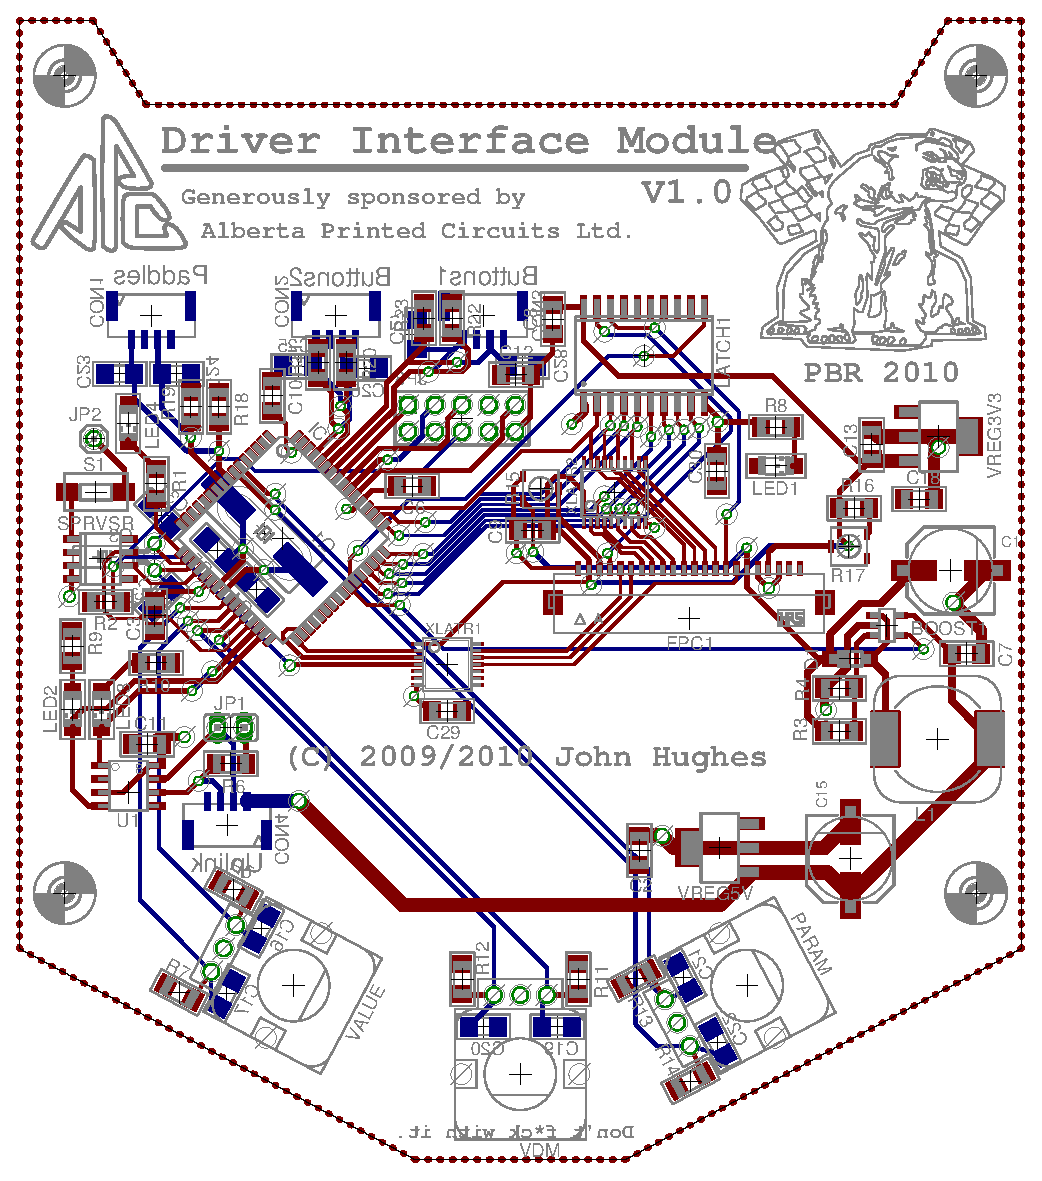
\includegraphics[width=3.5in,keepaspectratio]{implementation/figures/driver_interface_layout.eps}
  \caption{Board layout for the Telemetry module, exported from Eagle CAD.}
  \label{fig:driver_interface_layout}
\end{figure}

\subsection{Module Construction}

The printed circuit boards were manufactured by Alberta Printed Circuit (APCircuits), Ltd., who kindly sponsored the project. From the PCB layouts created in Eagle CAD, industry-standard GERBER-format files were generated and sent electronically to APCircuits. Figure \ref{fig:empty_pcbs} shows a photograph of the four empty PCBs after they were manufactured.

All four modules were populated and soldered by hand. Counter-intuitively, we found soldering the surface mount components with many leads to be easier than their through-hole counterparts. Initially we attempted to use paste stencils laser-cut out of mylar to apply the solder, in a process similar to that used in industry, however we found that for the relative incomplexity of our PCBs this was not of great aide. In the final manufacturing process, several steps were taken to populate each module:

\begin{enumerate}
  \item Once the circuit boards had arrived from manufacture, simple electrical tests were made to validate the construction: point to point checks of the ground and VCC planes were checked for continuity.
  \item An alchol-based circuit board cleaner was used to clean the surface of the boards of any contaminants.
  \item Solder paste was applied using a syringe individually to the large pads of resistors and capacitors, and in a thin strip across a line of smaller pads for the larger components.
  \item Individual components were placed on the pads with tweezers. The previously applied solder paste served as a slight adhesive.
  \item The entire board was placed in a toaster oven for approximately 7 minutes. Two-minute warm up and cool down periods were used before and after a 3 minute maximum tempurature reflow phase. The warm-up period served to evaporate the solvents in the solder paste, while the gradual cool down was performed to avoid thermal shock.
\end{enumerate}

\begin{figure}[h]
 \centering
 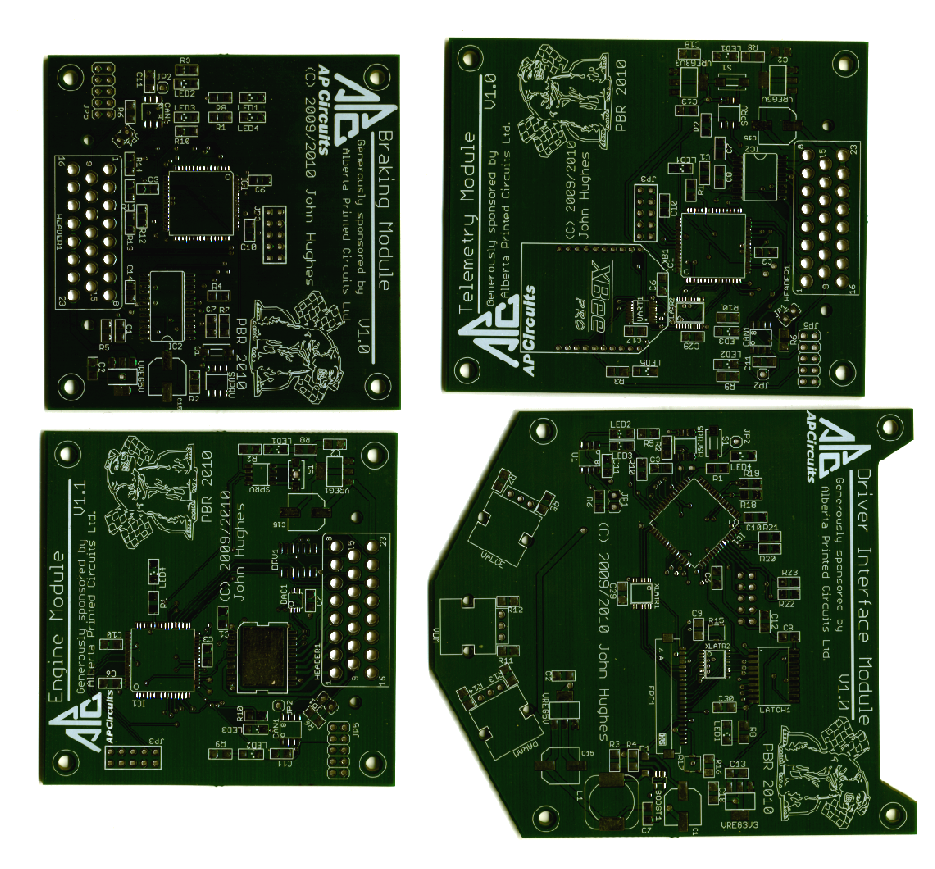
\includegraphics[width=5in,keepaspectratio]{implementation/figures/empty_pcbs.eps}
 \caption[Empty circuit boards after manufacturing.]{Empty circuit boards after manufacturing. Clockwise: Braking module, Telemetry module, Driver Interface module, and Engine and Transmission module}
 \label{fig:empty_pcbs}
\end{figure}

Color photographs of each completed module are shown in the relevant sections discussing them.
\section{Common Software Implementation\label{sec:Software-Implementation}}


\subsection{Methodology}


\subsection{Toolchain}


\subsection{Common Low-Level Drivers}


\subsubsection{CAN Driver}


\subsubsection{EEPROM Driver}


\subsubsection{SPI Driver}
\section{Engine and Transmission Module}

The engine and transmission module implements the design specified in Sec.\ \ref{sec:engine_transmission_design}. The hardware and software aspects of this module's implementation are discussed in this section.

\subsection{Hardware}

In addition to the base system hardware common to all modules described in Sec.\ \ref{sec:base_system_hardware}, 3 additional hardware components were added. The high-current solenoid drivers specified in the design in Sec. \ref{sec:design_engine_transmission_hardware} were implemented with a single SPI capable octal \emph{low-side solenoid driver}. This driver chip responds to commands over SPI, and switches the low side output pins accordingly. It includes flyback protection circuitry to squash voltage spikes from the inductive load of the solenoid, and can also detect electrical shorts. Additionally, a CMOS buffer chip was added to interface the discrete pins on the ECU (described in Sec.\ \ref{sec:ecu_background_discrete_inputs}), and an SPI capable DAC was added to output the \unit{0-5}{\volt} signal required for setting the traction control slip percentage.

\begin{figure}[H]
\centering
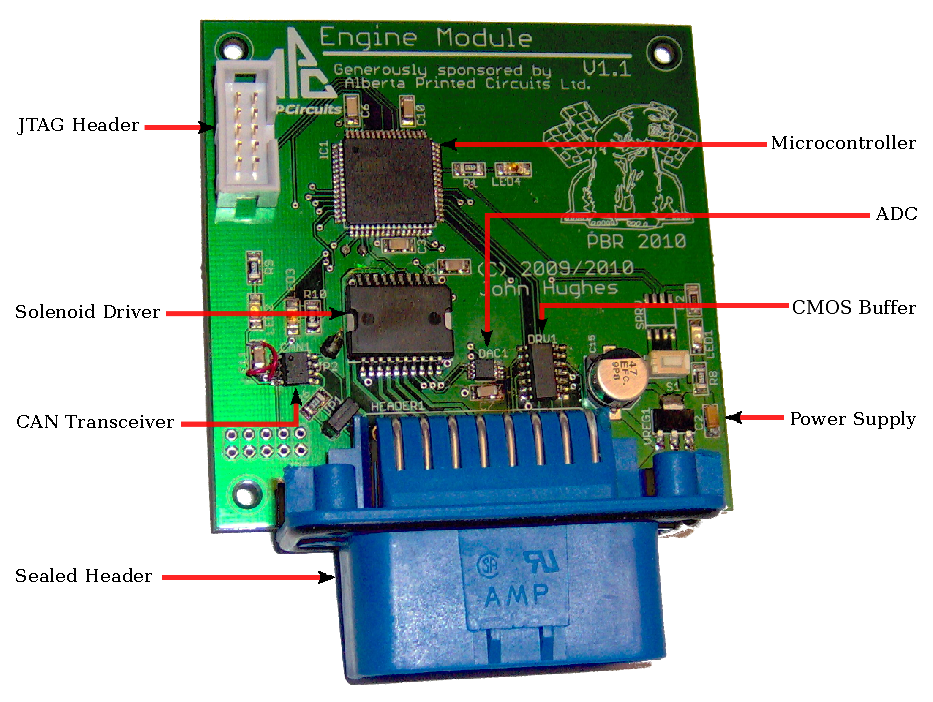
\includegraphics[scale=1]{implementation/figures/engine_transmission_pcb}
\caption{Populated Engine and Transmission module PCB.}
\label{fig:engine_transmission_pcb}
\end{figure}

Figure \ref{fig:engine_system_overview} shows a block-level diagram of the hardware implementation of the engine and transmission module, including the specific components chosen for the imlementation. A list of the components additional to the base system hardware can be found in Table \ref{tab:engine_transmission_module_components}. Descriptions of these components are in the following sections.

\begin{figure}[H]
\centering
\begin{tikzpicture}[auto, node distance=3.5cm, draw=black!70, >=stealth']
  \node [block, name=at90] {AT90CAN};
  \node [block, name=dac, left of=at90] {TLV5623 DAC};
  \node [block, name=driver, right of=at90] {L9822E Solenoid Driver};
  \node [block, name=can, below of=at90, above=0.5cm] {MCP2551 CAN Transceiver};
  \node [block, name=buf, left of=can] {74LVC07 Buffer};

  \node [block, name=ecu, rotate=90, minimum width=8em] at ($(dac.west)!0.5!(buf.west)+(-1.25cm,0)$) {ECU};
  \node [block, name=solenoids, right of=driver, left=-0.75cm] {Solenoids};
  \node [block, name=feedback, below of=solenoids, above=0.75cm, text width=2.2cm, inner sep=0.05cm] {Position Transducers};

  \path (at90.north)+(0.0,+0.4) node (title) {Engine Module};

  \begin{pgfonlayer}{background}
    \path (dac.north west)+(-0.3,0.7) node (a) {};
    \path (can.south -| driver.east)+(+0.3,-0.2) node (b) {};
    \path[module] (a) rectangle (b);
  \end{pgfonlayer}

  \node [bus, name=can1, below of=can, label=below:CAN Bus, above=2.0cm] {CAN Bus};
  \node [bus, name=can2, left of=can1] {};
  \node [bus, name=can3, right of=can1] {};

  \draw [-, line width=3pt] (can) -- (can1);
  \draw [-, line width=3pt] (can1) -- (can2);
  \draw [-, line width=3pt] (can1) -- (can3);

  \draw [->, thick] (driver) -- (solenoids);

  \draw [->, thick] (at90) -- node[above] {SPI} (driver);
  \draw [<->, thick] (at90) -- (can);
  \draw [->, thick] (at90) -- node[above] {SPI} (dac);
  \draw [->, thick] ($(at90.west)+(0,-0.3)$) to[myncbar, arm=0.5cm, angle=180] (buf);
  \draw [<-, thick] ($(at90.east)+(0,-0.3)$) to[myncbar, arm=0.5cm] (feedback);

  \draw [->, thick] (dac.west) to[myncbar, arm=0.2cm, angle=180] ($(ecu.south)+(0,0.5)$);
  \draw [->, thick] (buf.west) to[myncbar, arm=0.2cm, angle=180] ($(ecu.south)+(0,-0.5)$);
% 
% 
%   \draw [-, line width=2pt] (can1) -- (can2);
%   \draw [-, line width=2pt] (can2) -- node[rotate=90, above] {CAN Bus} (can3);
%   \draw [-, line width=2pt] (can3) -- (can4);
% 
%   \node [bus, above of=can1, below=1cm] (tip1) {};
%   \node [bus, below of=can4, above=1cm] (tip2) {};
%   \draw [-, densely dashed, line width=2pt] (can1) -- (tip1);
%   \draw [-, densely dashed, line width=2pt] (can4) -- (tip2);
% 
%   \node [block, right of=can2, right, text width=8em] (engine) {Engine Module};
%   \node [block, right of=can3, right, text width=8em] (ecu) {ECU};
% 
%   \node [block, right of=engine, right, text width=8em] (starter) {Starter System};
%   \node [block, right of=ecu, right, text width=8em] (intake) {Intake System};
%   \node [block, above of=starter, text width=8em] (transmission) {Transmission System};
% 
%   \draw [<->] (engine) -- (ecu);
%   \draw [<->] (engine.south east) -- (intake.north west);
%   \draw [<->] (engine) -- (starter);
%   \draw [<->] (engine.north east) -- (transmission.south west);
% 
%   \draw [<->, line width=2pt] (can2) -- (engine);
%   \draw [<->, line width=2pt] (can3) -- (ecu);
\end{tikzpicture}
\caption{Engine and transmission module hardware overview.}
\label{fig:engine_system_overview}
\end{figure}

\begin{table}
  \caption{Engine and Transmission module components.\label{tab:engine_transmission_module_components}}
  \centering
  \begin{tabular}{|c|c|c|}
    \hline 
    Part & Manufacturer & Part Number\tabularnewline 
    \hline \hline
    Solenoid Driver & ST Microelectronics & L9822E \tabularnewline
    \hline
    Digital to Analogue Converter & Texas Instruments & TLV5623C \tabularnewline
    \hline
    Hex CMOS Buffer & Texas Instruments & 74LVC07A \tabularnewline
    \hline
  \end{tabular}
\end{table}


\subsubsection{High Current Solenoid Driver}

In order to meet the requirement of being able to energize the multiple solenoids specified in the design, an 8-way solenoid driver component from ST Microelectronics was chosen. The LT9822E provides a simple SPI interface for the microcontroller to talk to, and also takes care of possible flyback from the solenoids with built-in clamping diodes.

Using this single component strongly reduces the complexity of the output stage of the circuit, since multiple discrete high-current transistors were not needed.

\subsubsection{Input Buffers}


\subsubsection{Traction Control Analogue Output}

In order to generate a 0-5V analogue signal for the ECU's traction slip ratio input, as was described in Sec. \ref{sec:background_ecu_data_interfaces}, a simple SPI interfaced digital to analogue converter (DAC) from Texas Instruments was introduced. The TLV5623 outputs \unit{0-5}{\volt} analogue signal that varies with the digital input.

The output voltage from the DAC can be determined by the following equation:

\begin{equation}
V_{out}=2\cdot{V_{ref}}\,\frac{Code}{2^{n}}\,\volt
\end{equation}

where $V_{ref}$ is the reference voltage input to the chip, $n=8\,(bits)$, and $Code$ is the digital input value ranging from $0$ to $2^{n-1}$. Since we want to output $\unit{5}{\volt}$ at fullscale input,

\begin{equation}
2\cdot{V_{ref}}\,\frac{2^{7}}{2^{8}}=V_{ref}=\unit{5}{\volt}
\end{equation}.

The DC input resistance $R_{in}$ on the traction cut input pin on the ECU was measured using a series resistor with the input terminal to be $R_{in}\approx\unit{155}{\kilo\ohm}$. The output current of the DAC therefore will be at most $I_{out}=\frac{5v}{155k}\approx\unit{32.26}{\micro\ampere}$.

\subsection{Software}

<Software interface map>


\subsubsection{Transmission Manager}


\subsubsection{Intake Manager}


\subsubsection{Starter Manager}


\subsubsection{Event Scheduler}


\subsubsection{CAN Interface}

<Data flow diagram>


\subsubsection{PWM Generator}

An efficient method was devised to generate 2 synchronized PWM signals from the L9822E driver chip. The $32\, kHz$ external crystal was used as the input to the 8-bit TIM2 timer periferal on the microcontroller. The input to the timer was first scaled by 8 which provided a timebase:
\begin{equation}
TB=\frac{32.768\, kHz}{8}=4.096\, kHz
\end{equation}

The timebase period is then given by:
\begin{equation}
\frac{1}{TB}\approx244\,\mu{S}
\end{equation}

We then define a constant scaling factor for the PWM generator:
\begin{equation}
{PWM\_DUTY\_SCALE}=\frac{T_{PWM}}{TB}\approx205
\end{equation}

By loading the timers compare register with with a value scaled with the constant scaling factor, we can cause the timer to generate an interrupt precisely when a level change in the PWM is required.

When generating 2 waveforms with the same timer periferal, 8 combinations of duty cycles of channels A and B were identified, and can be seen in Figure \ref{fig:pwm_cases}.

Since the waveforms are synchronized, it can be seen that there are only 2 cases where 3 transitions per period are required, corresponding to \ref{fig:pwm_cases_1} and \ref{fig:pwm_cases_2}. This happens when both channels have $0<Duty<100\%$. 2 cases are also apparent when no transitions are required, shown in \ref{fig:pwm_cases_7} and \ref{fig:pwm_cases_8}.

An efficient generating routine was constructed to effect the level transitions and to reset the timer to interrupt at the next transition. For the two cases requiring 3 transitions per period, the timer interrupts 3 times per period. For the two cases where both channels have duty cycle between 0 and 100\%, the routine still interrupts once to allow for a change in duty cycle. For the rest of the cases described, the timer only interrupts twice per PWM period.

\begin{figure}[ht]
  \centering
  \subfigure[Case 1]
  {
    \label{fig:pwm_cases_1}
    \begin{tikztimingtable}
      $PWM_A$		& G 4H 4L \\
      $PWM_B$		& G 2H 6L \\
    \end{tikztimingtable}
  }
  \subfigure[Case 2]
  {
  \label{fig:pwm_cases_2}
  \begin{tikztimingtable}
    $PWM_A$		& G 4H 4L \\
    $PWM_B$		& G 6H 2L \\
  \end{tikztimingtable}
  }
  \subfigure[Case 3]
  {
  \label{fig:pwm_cases_3}
  \begin{tikztimingtable}
    $PWM_A$		& G 4H 4L \\
    $PWM_B$		& 8L \\
  \end{tikztimingtable}
  }
  \subfigure[Case 4]
  {
  \label{fig:pwm_cases_4}
  \begin{tikztimingtable}
    $PWM_A$		& G 4H 4L \\
    $PWM_B$		& G 8H G \\
  \end{tikztimingtable}
  }
  \subfigure[Case 5]
  {
  \label{fig:pwm_cases_5}
  \begin{tikztimingtable}
    $PWM_A$		& G 8H G \\
    $PWM_B$		& G 4H 4L \\
  \end{tikztimingtable}
  }
  \subfigure[Case 6]
  {
  \label{fig:pwm_cases_6}
  \begin{tikztimingtable}
    $PWM_A$		& 8L \\
    $PWM_B$		& G 4H 4L \\
  \end{tikztimingtable}
  }
  \subfigure[Case 7]
  {
  \label{fig:pwm_cases_7}
  \begin{tikztimingtable}
    $PWM_A$		& 8L \\
    $PWM_B$		& 8L \\
  \end{tikztimingtable}
  }
  \subfigure[Case 8]
  {
  \label{fig:pwm_cases_8}
  \begin{tikztimingtable}
    $PWM_A$		& G 8H G \\
    $PWM_B$		& G 8H G \\
  \end{tikztimingtable}
  }
  \caption{PWM Cases (1 period shown).}
  \label{fig:pwm_cases}
\end{figure}

\subsubsection{Main Control Loop}
\section{Braking Module}

The Braking module implements the design specified in Sec.\ \ref{sec:Braking-Module-Design}. The hardware and software aspects of this module's implementation are discussed in this section.

\begin{figure}[h]
\centering
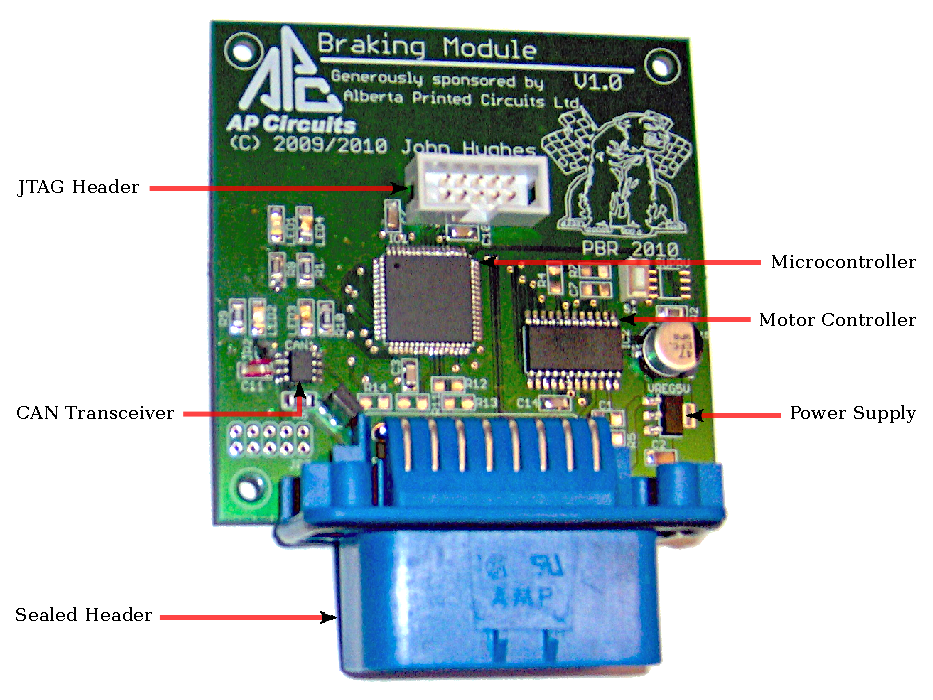
\includegraphics[scale=1]{implementation/figures/braking_pcb}
\caption{Populated Braking module PCB.}
\label{fig:braking_pcb}
\end{figure}

\subsection{Hardware}

The braking module implementation was the simplest of the 4 modules in terms of electrical design. Only one special hardware component was required, namely the stepper motor driver. This is summarized in Table \ref{table:braking_module_components}.

Figure \ref{fig:braking_pcb} shows a photograph of the completed braking module circuit board, with all components soldered on. The simplicity of the electrical design is reflected in the fact that no additional corrections (other than for the CAN transceiver) were required for the module to be 100\% operational.

\begin{table}
  \caption{Braking module components.\label{table:braking_module_components}}
  \centering
  \begin{tabular}{|c|c|c|}
    \hline 
    Part & Manufacturer & Part Number\tabularnewline 
    \hline \hline
    Stepper Motor Controller/Driver & Allegro Microsystems & A3967 \tabularnewline
    \hline
  \end{tabular}
\end{table}

\subsubsection{Stepper Motor Driver}

In order to meet the design goal of having the implementation be flexible in terms of which stepper motor would be used in the system, a current-sensing stepper motor controller/driver component was used in the circuit design. The current sense capability allows us to fix the input voltage in the circuit design, and afterwards adjust the current drive by changing resistor values in the current-sense feedback loop. 

The A3967 ``Micro-stepping Driver with Translator'' was chosen to drive the stepper motor for several reasons. The A3967 integrates a micro-stepping controller with dual H-Bridge output stages into one package. This simplified the potential circuit design. The H-Bridge output transistors can supply up to $\pm\unit{750}{\milli\ampere}$ of current at up to \unit{30}{\volt} \cite{A3967}. 

\paragraph{Current Control}
\nomenclature{$R_{sense}$}{Value of the current sense resistors in the Braking Module's stepper motor circuit.}
\nomenclature{$I_{TRIP}max$}{Maximum current allowed to flow into the Braking Module's stepper motor before the PWM circuit shuts the output stage off.}

The current control feature of the A3967 works by sensing the current through a sense resistor, $R_{sense}$, and varies the duty cycle of a fixed off-time PWM circuit, which controls the output from the H-Bridge stages.

The value of the sense resistor was determined by an equation recommended in the datasheet:
\begin{equation}
R_{sense}=\frac{0.5}{I_{TRIP}max}
\end{equation}
where $I_{TRIP}max$ is the maximum current allowed to flow into the motor before the PWM circuit shuts the output stage off.

The actual value of $R_{sense}$ used for bench testing the Braking module was \unit{2}{\ohm}, which allows \unit{250}{\milli\ampere} output current. This was suitable for the stepper motor used in testing.

\subsubsection{Analogue-to-Digital Converter}

The AT90CAN128's built-in analogue-to-digital converter was used to measure the analogue signals from the brake pressure transducers.

\subsubsection{End-of-Travel Microswitches}



\subsection{Software}


\subsubsection{Bias Library}


\paragraph{Bias Position Request}

<Position request flow chart>


\paragraph{Bias Calibration}

<Calibration flow chart>


\subsubsection{Pressure Library}


\paragraph{Periodic Pressure Output}


\paragraph{Pressure Calibration}

<Calibration flow chart>


\subsubsection{CAN Interface}

<Data flow diagram>


\subsubsection{Main Control Loop}
\section{Telemetry Module}

The Telemetry module implements the design specified in Sec.\ \ref{sec:Telemetry-Module-Design}. The hardware and software aspects of this module's implementation are discussed in this section.

\begin{figure}[H]
\centering
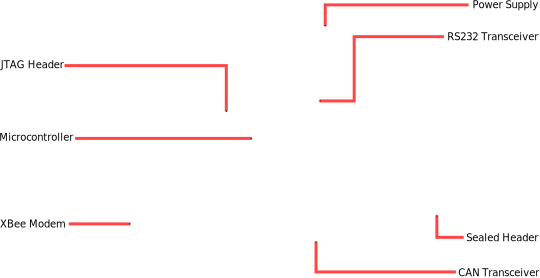
\includegraphics[scale=1]{implementation/figures/telemetry_pcb.eps}
\caption{Populated telemetry module PCB.}\label{fig:telemetry_pcb}
\end{figure}

\subsection{Hardware}

In addition to the base system hardware common to all modules described in Sec.\ \ref{sec:base_system_hardware}, several additional components were required in the implementation of the Telemetry module. A block diagram of the Telemetry module hardware implementation is shown in Fig.\ \ref{fig:telemetry_hardware_block}. The additional components are an XBee-PRO wireless mode, MAX232 RS-232 transceiver, MAX3100 external UART, an LTI1521 \unit{3.3}{\volt} linear voltage regulator, and an ST2378E 8-bit level translator. These additional components are listed in Table \ref{tab:telemetry_module_components} and will be described further in this chapter.

\begin{figure}[H]
\centering
\begin{tikzpicture}[auto, node distance=4cm, draw=black!70, >=stealth']
  \node [block, name=max3100] {Max3100 SPI UART};
  \node [block, name=at90, right of=max3100] {AT90CAN};
  \node [block, name=rs232, right of=at90] {Max232 RS232 Transceiver};
  
  \node [block, name=can, below of=at90, above=1cm] {MCP2551 CAN Transceiver};
  \node [block, name=modem, left of=can] {XBee Modem};
  
  \node [block, name=ecu, right of=rs232] {ECU};
  \node [block, name=dac, below of=ecu, above=1cm] {DAC};

  \path (at90.north)+(0.0,+0.4) node (title) {Telemetry Module};

   \begin{pgfonlayer}{background}
       \path (max3100.north west)+(-0.3,0.7) node (a) {};
       \path (can.south -| rs232.east)+(+0.3,-0.2) node (b) {};
       \path[module] (a) rectangle (b);
   \end{pgfonlayer}

  \node [bus, name=can1, below of=can, label=below:CAN Bus, above=2.5cm] {CAN Bus};
  \node [bus, name=can2, left of=can1] {};
  \node [bus, name=can3, right of=can1] {};

  \draw [-, thick] (modem.west) -| ($(modem.west)+(-0.8,0.2)$) \antenna;

  \draw [-, line width=3pt] (can) -- (can1);
  \draw [-, line width=3pt] (can1) -- (can2);
  \draw [-, line width=3pt] (can1) -- (can3);

  \draw [<->, thick] (at90) -- node[] {SPI} (max3100);
  \draw [<->, thick] (max3100) -- node[text width=2cm] {Serial} (modem);
  \draw [<->, thick] ($(at90.east)+(0,0.1)$) to[myncbar, arm=1cm] ($(rs232.north west)+(0,-0.5)$);
  \draw [<-, thick] ($(at90.east)+(0,-0.1)$) to[myncbar, arm=1cm] ($(rs232.south west)+(0,+0.5)$);

  \draw [<->, thick] ($(rs232.north east)+(0,-0.5)$) to[myncbar, arm=1cm] (ecu);
  \draw [<-, thick] ($(rs232.south east)+(0,0.5)$) to[myncbar, arm=1cm] (dac);

  \draw [<->, thick] (at90) -- (can);

%  \draw [<->, thick] (modem) -- node[] {} (telemetry);
%  \draw [<->, thick] (telemetry) -- node[] {RS232} (ecu);
%  \draw [<->, thick] (telemetry) -- node[] {RS232} (daq);
%  \draw [-, thick] (modem) -- node[text width=1.5cm] {} (ant) \antenna;
\end{tikzpicture}
\caption{Block Diagram, Wireless Telemetry Module.\label{fig:telemetry_hardware_block}}
\end{figure}

\begin{table}[H]
  \caption{Wireless Telemetry Module Components\label{tab:telmetry_module_components}}
  \centering
    \begin{tabular}{|c|c|c|}
      \hline 
      Part & Manufacturer & Part Number\tabularnewline
      \hline
      \hline
      XBee-PRO OEM Module & Digi International & XBee-PRO\tabularnewline
      \hline 
      Dual RS-232 Transceiver & Maxim Electronics & MAX232\tabularnewline
      \hline 
      SPI-capable UART chip & Maxim Electronics & MAX3100\tabularnewline
      \hline 
      300mA Low Dropout Regulator & Linear Technology & LT1521\tabularnewline
      \hline
      8-bit dual-supply level translator & ST Microelectronics & ST2378E\tabularnewline
      \hline
    \end{tabular}
\end{table}

\subsubsection{Dual RS-232 Transceiver}

The ECU and the DAQ modules connect to the telemetry board with specialized cables that connect to the wiring harness. The ECU and DAQ interface with two built-in USART ports on the AT90CAN128 micro-controller. A MAX232 dual RS-232 trasceiver chip was used in the design to interface the built-in UARTS on the AT90CAN128 with the line levels expected by the serial ports on the ECU and DAQ.

\subsubsection{XBee-PRO Wireless Modem and External SPI UART}

To meet the range and data throughput requirements for the telemetry system, an XBee-PRO wireles modem was used. The XBee requires \unit{3.3}{\volt} I/O levels and power supply, and so a second linear voltage regulator was used in the design, the LT1521 from Linear Technology. Since the AT90CAN129 has only 2 built-in UARTS that were used for the RS232 interfaces to the ECU and DAQ, an third external UART was added to the design. The MAX3100 is a SPI-interfaced UART with an 8 word deep FIFO buffer. It is interfaced to the AT90CAN128's SPI pins and has an active-low IRQ line connected to external interrupt line EXT7 on the microcontroller.

The wireless transmitter consumes at most \unit{215}{\milli\ampere} of current during transmit \cite{XBeeManual}. Since the common module hardware only provides power for 5V devices, the telemetry module has a second LDO regulator providing \unit{3.3}{\volt}. A separate antenna port is connected to the modem and mounted in the side of the module enclosure.

Since the XBee, MAX3100, and AT90CAN128 are operating at different logic levels, a dual-supply level translator was used. Signals between the XBee, MAX3100, and the low supply voltage side of the level translator use \unit{+3.3}{\volt} logic, while signals between the AT90CAN128 and the high supply voltage side of the level translator use \unit{+5}{\volt} logic.

\subsection{Software}

The primary objective of the software running on the Telemetry Module is to push data around from various sources to various sinks. An overview of the Telemetry module's system software can be seen in Fig.\ \ref{fig:telemetry_software_implementation}. A layer of software drivers interacts directly with the hardware, providing an easy-to-use interface for the specific system software to use. Interrupt-driven USART drivers were written for the on-board USARTs of the AT90CAN128, as well as the MAX3100 external UART.

Three major libraries 

Nearly 3000 lines of c code were written by us for the Telemetry modules' system software. 3800 lines of code were also contributed by David Schilling for the DAC library.

\begin{figure}[H]
\centering
\begin{tikzpicture}[auto, node distance=2cm, draw=black!70, >=stealth']
%  \draw[help lines] (-3,-5) grid (8,2);
  
  % Usart0 section
  \node [blue shiny, rectangle, minimum width=2cm] (usart0) {UART0};
  \node [blue shiny, rectangle, above of=usart0, node distance=1cm] (ecu) {ECU};

  \node [red shiny, rectangle, below of=usart0, right=-1cm, node distance=1cm] (usart0_rx) {Rx};
  \node [red shiny, rectangle, below of=usart0, left=-1cm, node distance=1cm] (usart0_tx) {Tx};

  \draw [<->] (ecu) to (usart0);
  \draw [<-] (usart0_rx) -- ($(usart0.south west)!(usart0_rx.north)!(usart0.south east)$);
  \draw [->] (usart0_tx) -- ($(usart0.south west)!(usart0_tx.north)!(usart0.south east)$);
  
  % Max3100 section
  \node [blue shiny, rectangle, minimum width=2cm, right of=usart0, node distance=3cm] (max3100) {MAX3100};
  \node [blue shiny, rectangle, above of=max3100, node distance=1cm] (xbee) {Xbee};
  \node [blue shiny, rectangle, below of=max3100, above=-0.3cm, left=0.25cm, node distance=0, font=\tiny, inner sep=0.075cm] (max3100_rx_hw) {Rx};

  \node [red shiny, rectangle, below of=max3100, right=-1cm, node distance=1cm] (max3100_rx) {Rx};
  \node [red shiny, rectangle, below of=max3100, left=-1cm, node distance=1cm] (max3100_tx) {Tx};

  \draw [<->] (xbee) to (max3100);
  \draw [<-] (max3100_rx) -- ($(max3100_rx_hw.south west)!(max3100_rx.north)!(max3100_rx_hw.south east)$);
  \draw [->] (max3100_tx) -- ($(max3100.south west)!(max3100_tx.north)!(max3100.south east)$);

  \node [red shiny, rectangle split, rectangle split parts=3, below of=max3100, text width=1.8cm, font=\scriptsize, text centered,
	  minimum width=2cm, anchor=base] (xbee_library)
    {XBee Library
      \nodepart{second} Packetizer
      \nodepart{third} Packet Buffer};

  %\node [red shiny, rectangle, below of=packetizer, node distance=1cm, minimum width=2cm,
%	  text width=1.75cm, font=\scriptsize, text centered] (packet_buf) {Rx Packet Buffer};

  \draw [->] (max3100_rx) -- ($(xbee_library.north west)!(max3100_rx.south)!(xbee_library.north east)$);
  \draw [<-] (max3100_tx) -- ($(xbee_library.north west)!(max3100_tx.south)!(xbee_library.north east)$);

  % Usart1 section
  \node [blue shiny, rectangle, minimum width=2cm, right of=max3100, node distance=3cm] (usart1) {UART1};
  \node [blue shiny, rectangle, above of=usart1, node distance=1cm] (dac) {DAC};

  \node [red shiny, rectangle, below of=usart1, right=-1cm, node distance=1cm] (usart1_rx) {Rx};
  \node [red shiny, rectangle, below of=usart1, left=-1cm, node distance=1cm, dashed] (usart1_tx) {Tx};

  \draw [<->] (dac) to (usart1);
  \draw [<-] (usart1_rx) -- ($(usart1.south west)!(usart1_rx.north)!(usart1.south east)$);
  \draw [->, dashed] (usart1_tx) -- ($(usart1.south west)!(usart1_tx.north)!(usart1.south east)$);

  \node [red shiny, rectangle split, rectangle split parts=4, below of=usart1, text centered, minimum width=2cm, anchor=base, text width=1.85cm, inner xsep=0, font=\scriptsize] (dac_library)
    {DAC Library
      \nodepart{second} Buffer
      \nodepart{third} Decoder
      \nodepart{fourth} Encoder};

  \draw [->] (usart1_rx) -- ($(dac_library.north west)!(usart1_rx.south)!(dac_library.north east)$);
  \draw [<-, dashed] (usart1_tx) -- ($(dac_library.north west)!(usart1_tx.south)!(dac_library.north east)$);

  % CAN stuff
  \node [blue shiny, rectangle, minimum width=2cm, right of=usart1, node distance=3cm] (can) {CAN};
  \node [red shiny, rectangle, minimum width=2cm, below of=can, node distance=1cm] (can_driver) {Driver};

  \node at (dac_library.third split -| can_driver)
	    [red shiny, rectangle, minimum width=2cm, text width=1.85cm, font=\scriptsize, text centered] (can_library) {Telemetry CAN Library};

  \draw [<->] (can) -- (can_driver);
  \draw [<->] (can_driver) -- (can_library);

  \draw [->] (dac_library.third east) -- ($(can_library.north west)!(dac_library.third east)!(can_library.south west)$);
  \draw [<-] (dac_library.fourth east) -- ($(can_library.north west)!(dac_library.fourth east)!(can_library.south west)$);

  % Now for the rest of the connections
  \draw [->] (xbee_library.third west) -| (usart0_tx);
  \draw [<-] (xbee_library.second west) -| (usart0_rx);
  \draw [->] (dac_library.second west) to node [name=mid1] {} (xbee_library.second east);
  \draw [->] (dac_library.fourth west) -| (mid1);

  \node [left of=usart0, node distance=3cm, minimum width=3.5cm] (perifs) {Module Periferals};
  \node [below of=perifs, node distance=1cm, minimum width=3.5cm] (buffers) {Drivers/Buffers};
  \node [below of=buffers, node distance=1cm, minimum width=3.5cm] (libraries) {Libraries};

  \begin{pgfonlayer}{background}
    \path (perifs.north west)+(-0.0,0.1) node (a1) {};
    \path (can.south east)+(+0.1,-0.1) node (b1) {};
    \path[draw=blue!50!black!50, rounded corners=0.1cm] (a1) rectangle (b1);

    \path (buffers.north west)+(-0.0,0.1) node (a2) {};
    \path (can_driver.south east)+(0.1,-0.1) node (b2) {};
    \path [draw=red!50!black!50, rounded corners=0.1cm] (a2) rectangle (b2);

    \path (libraries.north west)+(-0.0,0.1) node (a3) {};
    \path (can_library.south east)+(0.1,-0.1) node (b3) {};
    \path [draw=red!50!black!50, rounded corners=0.1cm] (a3) rectangle (b3);
  \end{pgfonlayer}

  % Guide
  \node at ($(a3 |- b3)+(0.0,-0.1)$) [anchor=north west, blue shiny, minimum width=2cm] (hardware) {Hardware};
  \node [red shiny, right of=hardware, node distance=2.2cm, minimum width=2cm] (software) {Software};
  
\end{tikzpicture}

\caption{Telemetry software overview.}
\label{fig:telemetry_software_implementation}
\end{figure}

\subsubsection{Internal and External USART Drivers}

Software drivers for both the internal built-in USART periferals as well as the MAX3100 external UART were written in a similar fashion, and share the same software interfaces and buffering code. The drivers were written to utilize the hardware interrupts of the periferals to allow asynchronous sending and receiving of data. A statically allocated circular buffering approach was taken for both receiving and transmitting data. An abstracted flow chart of the USART interrupt handling is shown in Fig.\ \ref{fig:usart_driver_flow}.

\paragraph{MAX3100 SPI Interface}

The datahseet for the MAX3100 states that the minimum SPI Clock period is $t_{CP}=\unit{238}{\nano\second}$, which results in a maximum frequency of approximately $\unit{4.2}{\mega\hertz}$ \cite{MAX3100}. The SPI periferal was thus set to use 1/4 of the system clocks frequency resulting in $\unit{4}{\mega\hertz}$.

\begin{figure}[H]
\centering
\begin{tikzpicture}[auto, node distance=2cm, draw=black!70, >=stealth']
  \node [start] (int) {Interrupt};
  \node [decision, right of=int, right=0cm] (rx) {Rx Byte?};
  \node [block, below of=rx] (add) {Add to Rx buf.};

  \node [decision, right of=rx, right=0cm] (tx) {Tx Byte?};
  \node [block, below of=tx, text width=2.5cm, inner xsep=0pt] (remove) {Remove from Tx buf.};
  \node [end, right of=tx, right=0cm] (return) {Return};

  \draw [->] (int) -- (rx);
  \draw [->] (rx) to node [] {yes} (add);

  \draw [->] (rx) -- node [name=mid] {no} (tx);
  \draw [->] (add) -| (mid);

  \draw [->] (tx) to node [] {yes} (remove);
  \draw [->] (tx) -- node [name=mid2] {no} (return);
  \draw [->] (remove) -| (mid2);

\end{tikzpicture}
\caption{Basic USART interrupt flow diagram.}
\label{fig:usart_driver_flow}
\end{figure}

\subsubsection{Xbee Library}

In order to facilitate routing data to and from multiple sources and sinks, it was determined that the Xbee would need to be interfaced using the special "API" mode described in the Xbee documentation \cite{XBeeManual}. The API mode is characterized by a packet interface that needed to be implemented in software. A library was written to implement two critical pieces of functionality:

\begin{enumerate}
\item to set the modem into API mode operation and manage the modem's operating state;
\item and to send and receive packetized data from the modem on behalf of the user software as per the Xbee's API specification \cite{XBeeManual};
\end{enumerate}

The Xbee library implements the binary packet protocol described in the XBee manual, and is able to send and receive unicast and multicast packets. The driver is only capable of sending packets to 16-bit addresses. Full 64-bit address mode was not implemented as the address space was not required in our 3 node network. The driver is also capable of sending command-type packets to the modem and reading the response.

Managing the modem's state was implemented as a state machine. Since minimal functionality was required, only a handful of modem commands were implemented. The driver is able to push the modem into API mode, after which all communication is done using the packet interface.

The modem commands implemented are listed in Table \ref{tab:xbee_commands}.

\begin{table}
\caption{Implemented Xbee modem commands.\label{tab:xbee_commands}}
\centering{}
\begin{tabular}{|l|l|}
\hline 
Command & Description \tabularnewline
\hline
\hline
AP & Set and read the API mode state \tabularnewline
\hline
CH & Set and read the RF channel \tabularnewline
\hline 
ID & Set and read the PAN (Personal Area Network) ID \tabularnewline
\hline
MY & Set and read the modems local address \tabularnewline
\hline
\end{tabular}
\end{table}

Similar to the rest of the software drivers implemented, the Xbee library uses callbacks to provide the user software with incoming data. Function pointers are used to connect the library to a UART, which makes it possible to reconfigure the library to use a different USART on-the-fly.

\subsubsection{DAC Library}

To reduce the implementation work required by us, we asked David Schilling, a computer science student on the Formula SAE team, to write the DAC software library to read and write the DAC's serial format, given the requirements described in Section \ref{sec:Telemetry-Module-Design}.

The DAC library maintains it's own buffer of incoming DAC data. We also asked Dave to provide seperate functions for buffering incoming data, and for processing that data. This seperation allowed the library to be easily tied in with the rest of the system software on the telemetry module: adding a data to the DAC buffer occurs whenever the internal USART driver interrupts with a new byte, and processing is called from the mainline loop.

\subsubsection{Main Control Loop}
\section{Driver Interface Module}

The driver interface module implements the design specified in Sec.\ \ref{sec:Driver-Interface-Module}. The hardware and software are discussed in this section. Figure \ref{fig:driver_interface_pcb} shows a photo of the completely populated and debugged driver interface module PCB.

\begin{figure}[h]
\centering
\includegraphics[scale=1]{implementation/figures/driver_interface_pcb.eps}
\caption{Photograph of the populated driver interface module PCB.}\label{fig:driver_interface_pcb}
\end{figure}

\subsection{Hardware}

The driver interface module provides all of the support hardware needed for the LCD module to function. An \emph{FPC} connector, \emph{LCD bias boost converter}, \unit{+3.3}{\volt} power supply, latch, and level translators are all included in the module. Additionally, three rotary encoders are soldered onto the board. Connectors are soldered onto the back of the PCB to connect the steering wheel-mounted push buttons and paddles.

\subsubsection{LCD Module}

The LCD module used in the driver interface implementation is a pre-packaged LCD module from Newhaven Display. Along with the actual LCD panel, a built-in display controller chip and display RAM are included. Interfacing with the LCD module entails interfacing with it's controller chip, a SED1335 LCD controller IC from Seiko Epson Corporation. The controller chip handles all of the low level functionality of the LCD, such as generating pixel clocks and drawing to the screen from the LCD RAM. It also provides a character generator.

\subsubsection{LCD Bias Circuit}

The LCD screen requires a large bias voltage of \unit{+22}{\volt} to operate \cite{LCD_Module}. A Linear Technology LT1615 step-up DC/DC converter is used as the heart of a boost converter circuit to generate this bias voltage. The circuit schematic for the boost converter is shown in Fig.\ \ref{fig:lcd_boost_converter}.

\begin{figure}[H]
 \centering
 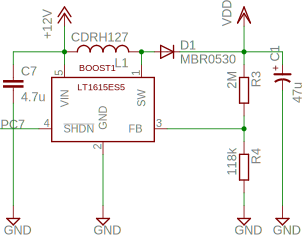
\includegraphics[scale=0.8]{implementation/figures/driver_interface_lcd_bias_circuit.eps}
 \caption{Schematic of the LCD boost converter circuit.}
 \label{fig:lcd_boost_converter}
\end{figure}

The data-sheet provides formulas for calculating the value of the inductor $L_1$. We calculated an inductor value of \unit{10}{\micro\henry}, which worked perfectly with the module.

To obtain a $V_{bias}$ of $+\unit{22}{\volt}$, two resistors in the bias circuit provide a voltage divided feedback path from the output to the \emph{FB} pin on the LT1615. The equation relating the output voltage with the resistor values is:

\begin{equation}
R_{3}=R_{4}\cdot\left(\frac{V_{bias}}{1.23}-1\right)
\end{equation}

 $R_{3}$ was chosen to be $\unit{2}{\mega\ohm}$ to limit current flowing from the output to ground, and a suitable $R_{4}$ of $\unit{118}{\kilo\ohm}$ was found.

\subsubsection{LCD Module Data Interface\label{sec:lcd_module_data_interface}}
\nomenclature{ALE}{Address Latch Enable}

The LCD's 8-bit interface can be connected to an external memory interface, making the LCD a memory-mapped peripheral. All of the read and write strobes are handled by the memory controller. The AT90CAN128's external memory interface uses a bank of eight pins as a multiplexed data and address bus. This bus must be demultiplexed in order to offer the separate address and data buses required by the LCD module. In operation, the micro-controller first puts out the address on the combined bus, followed by the data. A \emph{address latch enable} (ALE) signal to interface with an external latch to store the address bits.\cite{AT90CAN}.

\nomenclature{$t_{LHLL}$}{The Address Latch Enable pulse width on the AT90CAN128's external memory interface}
A fast octal D-Type latch from NXP, the 74LVC373A, is used to latch the address from the micro-controller. The width of the ALE pulse, $t_{LHLL}$, provided by the micro-controller is given as:

\begin{equation}
t_{LHLL}=t_{CLCL}-15\, \nano\second
\end{equation}

Here, $t_{CLCL}$ is the main clock period. With the main clock running at $\unit{16}{\mega\hertz}$, $t_{LHLL}=\unit{48}{\nano\second}$.

\nomenclature{$t_{CLCL}$}{The main system clock period on the AT90CAN128.}

The 74LVC373A latch from NXP requires a minimum LE pulse width of $\unit{4.5}{\nano\second}$, so is suitable as a demultiplexing interface.

The external memory on the AT90CAN128 starts at address 0x1100h, and there are two possible registers to read/write to on the LCD controller. The LCD controller therefore has it's single address select pin connected to the LSB of the address lines output from the latch. Since only two addresses are required, the upper 8 address lines of the external memory interface were not used.

\nomenclature{CS}{Chip Select}

A logical combination of the lower byte address lines are connected to the \emph{chip select} (CS) line on the LCD controller. Since the external memory controller only outputs it's control signals when the requested memory operation is referencing external memory, it is safe to ignore the upper byte address lines. The second bit of the address lines to the CS line on the LCD controller. The resulting operations when interacting with the LCD controller are summarized in Table \ref{tab:lcd_memory_map}.

\begin{table}[H]
\caption{List of memory addresses associated with the LCD interface.}
\centering{}
\begin{tabular}{|l|l|l|}
\hline 
Address  & Read Function  & Write Function\tabularnewline
\hline
\hline 
0x1101  & Status flag read  & Display data and parameter write\tabularnewline
\hline 
0x1102  & Display dada and cursor address read  & Command write\tabularnewline
\hline
\end{tabular}
\label{tab:lcd_memory_map}
\end{table}

\subsection{Software}

The software running on the driver interface module acts as a major source and sink of data on the network, sending driver commands out and listening to incoming diagnostic information. The majority of the software implemented is to support the LCD hardware. The software supporting the buttons, knobs, and paddles is very simple in comparison. The actual user interface and vehicle diagnostic mode managers are in the process of being implemented, however the main priority of the team has been to finish debugging the electro-pneumatic system and finish the transmission control software.

\subsubsection{LCD Module Library}

The LCD module library implements the entire command set of the SED1335. It is capable of initializing the LCD controller and screen, setting up different layers and cursors, and drawing strings and bitmaps. Additionally, more complex drawing operations are capable, such as the rendering of progress bars, underlines, a clock, and the signal strength indicator. It is also capable of generating a parameter menu system that allows the driver to scroll through the list of vehicle parameters to tune.

\subsubsection{Font Library}
\label{sec:lcd_module_font_loading}

The built-in font in the SED1335 LCD controller is only 5x7 pixels, and difficult to read. To display more readable text on the LCD screen, a custom 16x16 pixel fixed-width font for the character generator was developed. This font library implements a 43-character subset of the standard ASCII library, namely the capital letters A-Z, the numbers, and a few punctuation characters.

An 688x16 pixel image was created with an image manipulation program. 16 pixel wide blocks were sectioned off, and fixed width characters were drawn on the image at 16 pixel intervals. A small ``python'' script was written to pull the bitmap data out of the image and convert it into a constant array of bits suitable for a ``C'' header file.

The font library loads it's font data into the appropriate character generator RAM on the LCD at start-up. ASCII characters written to the character buffer in the LCD memory are drawn by the character generator and show up on the screen in the custom font. An image of the font used is shown in Fig.\ \ref{fig:driver_interface_font}.

\begin{figure}[htp]
 \centering
 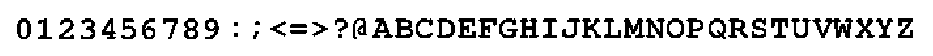
\includegraphics[scale=1]{implementation/figures/driver_interface_font.eps}
 \caption{Custom 16x16 pixel fixed-width font.}
 \label{fig:driver_interface_font}
\end{figure}

\subsubsection{I/O Library}

A small I/O Library was written to set up and manage the interrupts generated by the buttons, knobs, and paddles on the steering wheel. This library periodically polls the various inputs for status changes, and can signal the module software when a change of state has occurred.

\section{CAN Diagnostic Tool}
\label{sec:implementation_candt}

It was recognized early in the implementation that a means of testing the modules in isolation would be required. Access to the vehicle is limited during construction, and isolating a problem between four modules is an arduous task. With this in mind, we developed a CAN diagnostic tool to facilitate isolated testing of four modules.

The CAN diagnostic tool is a piece of software run on a third-party development board that allows the user to schedule a sequence of packets to be broadcast over the CAN bus. It also has provisions for relaying the bus activity back to the user.

\subsection{Hardware}

Our group received an Olimex AT90CAN128-based development board as a sponsorship donation from Optimal Microsystems. Like the four modules, the Olimex development board supports a JTAG-interface, and has D-sub type connectors on either end for RS-232 and CAN. An annotated photograph of the development board is shown in Fig. \ref{fig:impl_avr_can}.

\begin{figure}[H]
\centering
\includegraphics[scale=0.5]{implementation/figures/avr_can}
\caption{Photograph of the Olimex AT90CAN128 development module.}
\label{fig:impl_avr_can}
\end{figure}

\subsection{CAN Interface}

The CAN diagnostic tool communicates with the bus at a fixed 1 Mbit/s link speed, matching the standard used by the other modules. A standard D-sub type connector is used to interface with the bus. The pin-out for this connector is listed in table \ref{tbl:candt_pins}. 

\begin{table}[H]
  \caption{List of pins used by the DE-9 CAN connector.}
  \centering
  \begin{tabular}{|c|c|}
    \hline 
    Pin & Function \\
    \hline \hline
    1 & No Connection\\
    \hline    
    2 & CAN Low\\
    \hline    
    3 & Ground\\
    \hline    
    4 & No Connection\\
    \hline    
    5 & No Connection\\
    \hline    
    6 & Ground\\
    \hline    
    7 & Can High\\                 
    \hline    
    8 & No Connection\\
    \hline
    9 & Voltage In\\        
    \hline
  \end{tabular}
  \label{tbl:candt_pins}
\end{table}

By default, the board acts as a termination point for the CAN bus. The modules can be interfaced with the development module by connecting a bare female DE-9 shell with the appropriate leads soldered onto it. 

\subsection{Serial Interface}

The CAN diagnostic tool communicates with a user over the built-in serial interface. By default, the serial stream is configured to operate at 115,200 Kbps with 8 data bits, 1 stop bit, and no parity bit.

A simple software library links standard ``C'' input-output functions like ``\verb|printf()|'' and ``\verb|scanf()|'' to the internal UART, avoiding the need for interaction with the complicated UART library required by the other modules. 

Upon booting, the diagnostic tool outputs a welcome message over the serial link and indicates that it is waiting for a sequence to be input. Figure \ref{fig:candt_startup} shows a listing of this output as it would appear over the serial link.

\begin{figure}[H]
	\centering
	\makebox[\textwidth]{\hrulefill}
{\footnotesize	
	\begin{verbatim}
CAN-Tester 1.0 (c) 2009-2010 UMSAE
==================================

Ready for packet schedule.
	\end{verbatim}
}	
	\makebox[\textwidth]{\hrulefill}
	\caption{Output listing of the CAN diagnostic tool start-up sequence.}
	\label{fig:candt_startup}
\end{figure}

The packet schedule may now be input over the serial interface.

\subsection{User Interface}
\label{ref:candt_ui}

The packet schedule is a list of packets to be broadcast over the bus. A maximum of 100 packets can be scheduled at any given time. The parameters required for each packet are:

\begin{itemize}
	\item the \emph{packet type}, which specifies a data or remote request packet;
	\item the \emph{injection time}, which indicates the time at which the packet should be broadcast;
	\item the \emph{identifier mode}, which specifies if the packet uses the extended identifier feature;
	\item the \emph{identifier}, which defines the ID with which the packet will be broadcast;
	\item the \emph{data length}, which indicates how many bytes will be broadcast; and
	\item the \emph{data}, which includes the actual data bytes to be broadcast.
\end{itemize}

A detailed outline of the CAN diagnostic input protocol is outlined in Appendix \ref{apx:candt}. 

Once the packet schedule has been input by the user, it is relayed back over the serial link for verification by the user. Figure \ref{fig:candt_sched} shows a listing of the output seen for some arbitrary packet schedule.

\begin{figure}[H]
	\centering
	\makebox[\textwidth]{\hrulefill}
{\footnotesize	
	\begin{verbatim}
4 packets read from serial.

Packet Schedule:

 Time  (ms)   Direction    Format        ID        Type    DLC          Data                  
============ =========== ========== ============ ======== ===== =====================
 0000001000     Output    Standard   0x00000100    Data     1    0x01 
 0000002000     Output    Standard   0x00000105    Data     5    0x0102030405
 0000003000     Output    Extended   0x1FFFFFFF   Remote    0    
 0000004000     Output    Standard   0x000000FF    Data     8    0xFFFFFFFF04091A1C    
 
Press any key to start broadcasting.
	\end{verbatim}
}	
	\makebox[\textwidth]{\hrulefill}
	\caption{Output listing of an example packet scheduling interaction.}
	\label{fig:candt_sched}
\end{figure}

The CAN diagnostic tool then waits for the user to send any character over the serial line. At this time, the schedule is output onto the bus. A real-time display of the bus activity is relayed back to the user over the serial link. Outbound packets are also relayed back to the user as they are output. Figure \ref{fig:candt_output} shows a typical run. The tester will continue to output bus activity after it finishes uploading it's sequence. 

\begin{figure}[H]
	\centering
	\makebox[\textwidth]{\hrulefill}
{\footnotesize	
	\begin{verbatim}
Broadcasting...

Bus Activity:

 Time  (ms)   Direction    Format        ID        Type    DLC          Data                  
============ =========== ========== ============ ======== ===== =====================
 0000001000     Output    Standard   0x00000100    Data     1    0x01 
 0000001239     Input     Standard   0x000000AF    Data     3    0x1F999C  
 0000002000     Output    Standard   0x00000105    Data     5    0x0102030405
 0000003000     Output    Extended   0x1FFFFFFF   Remote    0    
 0000003004     Input     Extended   0x1FFFFFFF    Data     3    0x000000
 0000003099     Input     Extended   0x00000FFF    Data     1    0x0A 
 0000004000     Output    Standard   0x000000FF    Data     8    0xFFFFFFFF04091A1C    
	\end{verbatim}
}	
	\makebox[\textwidth]{\hrulefill}
	\caption{Output listing of an example CAN diagnostic tool run.}
	\label{fig:candt_output}
\end{figure}
 
\subsection{Packet Scheduler}

The packet scheduler handles the translation of input from the user into packets, and the actual queuing and dispatching of packets over the network. Each packet is described by a \emph{packet descriptor}, which is essentially a ``C'' structure that defines all of the packet parameters introduced in Sec. \ref{ref:candt_ui}. 

At the heart of the packet scheduler is a statically-allocated array of packet descriptors, called the \emph{packet queue}. The packet queue contains all the packets that are to be broadcast over the network, arranged by time of broadcast.

On start-up, the main software passes the serial input stream to the packet scheduler's main packet decoder function. Each new line of input is run through a decoding function that breaks the input format up into it's constituent parameters to form a packet descriptor. If the descriptor is valid, it is appended to the end of the packet queue.

Once the user is finished inputting the schedule, or the packet queue is full, the packet scheduler passes control back to the main program to wait for the user to request the broadcast begins.

Once broadcasting, the packet scheduler uses the internal timer of the micro-controller to interrupt the software every millisecond. During the interrupt service routine, the queue is checked to see if it is time to broadcast the next packet. If so, a message object is allocated on the CAN interface and is configured by the packet descriptor. Once the data payload is set, the packet is broadcast across the network. If any other packets are scheduled for the same time interval, they will be broadcast as well. 

Once the packet scheduler runs out of packets to broadcast, it stops it's timer and becomes dormant. A new packet schedule requires a hard reset of the development module.

\subsection{Bus Snooping}

Once the broadcast process begins, the CAN interface is configured to listen for any incoming packets. A general purpose callback is attached to the message object used to listen for packets. This callback prints out the packet's parameters to the serial stream. 

\subsection{Throughput Limitations}

It is possible that too many packets may arrive at once and overload the input stream. The longest output text is 104 bytes, or 832 bits. This corresponds to 138 possible lines of output per second, corresponding to 138 possible CAN packets per second. The shortest possible CAN packet is 41 bits, and the longest possible CAN packet is 576 bits, so the serial output limits the true bus speed to between $41*138 = 5658$ bps and $576 * 138 = 79488$ bps. This problem is not significant, as the modules do not typically generate more than 15 or 20 messages per second.



\chapter{Results and Discussion}


\section{Transmission}


\subsection{Shift Speed}


\subsection{Launch Control}


\subsection{Neutral Find}


\subsection{Anti-Stall}


\subsection{Electropneumatics}


\section{Intake}


\section{Starter}


\section{Braking}


\subsection{Bias Adjustment}


\subsection{Calibration}


\section{Telemetry}


\subsection{Data Interfaces}


\subsubsection{ECU }


\subsubsection{DAC }


\subsubsection{Wireless Data Link}


\section{Driver Interface}


\subsection{Driver Controls}


\subsection{Vehicle Dynamic Adjustment}


\subsection{Diagnostic Information}


\subsection{LCD Interface}

\subsubsection{Bench Test}

To verify the LCD data interface circuitry before the final Driver Interface module hardware had been completed, a bench test of the LCD module with an ARM7 development board was conducted. The same bus interface as designed in 

Once all the hardware bugs with the Driver Interface module had been corrected, it was possible to continue writing the LCD interfacing software that had been started during the LCD bench testing (described in Sec.\ \ref{FIXME!}.

\begin{figure}[h]
 \centering
 \includegraphics[width=6in,keepaspectratio]{experimental_results/figures/driver_interface_lcd.eps}
 \caption{Testing the LCD on the Driver Interface module.}
 \label{fig:driver_interface_lcd}
\end{figure}

\section{Electrical System and Harness}




\section{Implementation Issues Encountered}


\subsection{Hardware Implementation Issues}


\subsubsection{CAN Transciever Schematic Error}


\subsubsection{Driver Interface LCD Reset Line}


\subsubsection{Telemetry RS-232 Transciever Schematic Error}


\subsection{Interrupt Starvation on the Telemetry Module}

Although initial average data throughput rates for both the DAC and the ECU were measured as part of the research done at the beginning of the project, non-trivial buffering issues did arise in the implementation of the telemetry module software. After several weeks of work spent debugging throughput problems with the module software, and with the aide of a protocol analyser, the root of the problem was tracked down. The AT90CAN microcontroller's interrupt vectors are fixed at the factory, therefore the priority of interrupts on the microcontroller is fixed. Unfortunately this lead to a resource starvation issue. The MAX3100 UART uses an external interrupt line, which has priority over the internal UART interrupts. When there is data in the MAX3100's transmit buffer, it will starve the internal UART interrupt to a certain extent. This was investigated by saturating the MAX3100 output buffer with a constant stream of data, and then inputting some bytes to the internal UART. Single input bytes were read properly, but any long stream of incoming bytes (more than 4 in a row) would cause hardware input buffer overruns in the built-in UART, and incoming data would be lost.

\begin{figure}[ht]
  \centering
  \label{fig:ecu_data}
  \begin{tikztimingtable} %[timing/nice tabs]
    $ECU_{Rx}$ & Z 10D{Polling sequence (7 bytes)} 14F Z \\
    $ECU_{Tx}$ & 12Z 6D{Reply sequence} ;[dotted] 2D{...}; 5D{(539 bytes)} Z\\
    \extracode
      %\tableheader{Signal}{Timing}
      \tablerules
  \end{tikztimingtable}
  \caption{ECU Serial Data Example}
\end{figure}

Based on this knowledge, we were able to classify conditions where the software would be unable to accurately process the incoming data. Unfortunately the method that the ECU transmits it's data falls within this characterization. When the ECU is communicating with the DTASWin software, the software will send a handful of bytes (around 7) to the ECU, and the ECU will reply with one large packet of approximately 540 bytes. If the MAX3100 is transmitting a large amount of data when this large packet comes in, bytes will be lost from the interrupt starvation issue.

Having determined the problem, several options lay before us to resolve the issue:
\begin{itemize}
  \item By lumping the ISR handlers for both the internal UART and the MAX3100 together, it would be possible to conditionally alter the priority of the processing to allow the incoming data to take precedence. This would however override the natural encapsulation that the two drivers had, and would require writing specialized drivers for use only on the telemetry module.
  \item Throttling the transmission of data to the MAX3100 by sequenced enabling and disabling of the interrupt could also reduce the starvation issue, but getting the sequencing and timing right would be difficult and more than likely result in further problems.
\end{itemize}


\subsection{CAN Driver Problems}

%%% Shorten the running head so it doesn't collide in this chapter...
\fancyhead[L]{Automotive Network}

\chapter{Conclusions and Recommendations}

This chapter will outline the contributions of the project and summarize what was accomplished. Recommendations for future work for each of the four modules will also be made.

\section{Conclusions}

In this thesis we have discussed the goals, designs, and implementations of a network of four modules for the 2010 Formula SAE vehicle.

\begin{itemize}

  \item A novel pneumatic design was proposed to improve the actuation of the clutch and shift mechanisms of the transmission. A Simulink model was developed of this system, and the hardware and software basis for an on-car controller was designed and implemented. Additionally, driver interactions with the system have been detailed, and advanced controller functions designed.

  \item The first iteration of a braking module was designed and implemented allowing electronic control of the vehicles brake bias.

  \item A multiplexing telemetry module was designed and implemented allowing multiple data source on the vehicle to stream data to their proprietary PC software.

  \item The first iteration of a dynamic driver interface module was designed and implemented that allows drivers to control vehicle parameters at runtime.
  
\end{itemize}

\section{Recommendations for Future Work}

To further the goals set out in Ch.\ \ref{cha:goals}, and to generally improve upon what was accomplished during this project, the following items have been identified as recommendations for future work:

\subsection{Engine and Transmission}

Several engine and transmission goals are not realizable until the vehicle has been constructed. Once constructed, future work includes:

\begin{itemize}
  \item Identification of the model parameters within the actual electro-pneumatic system;
  \item Development of the electro-pneumatic controlling algorithms;
  \item Physical implementation of the electro-pneumatic actuation system;
  \item Physical implementation of the variable intake actuator.
\end{itemize}

\subsection{Braking}

The brake module has yet to be tested with the brake pedal assembly, as it has not yet been fabricated. Future work includes testing the bias adjustment and calibration procedures with the actual balance bar.

\subsection{Telemetry}

The telemetry module has yet to be field tested to determine if it meets the range requirements proposed. Future work includes testing the range of the telemetry module and its noise resilience at the Formula SAE competitions.

\subsection{Driver Interface}

At the time of project completion, the steering wheel had not yet been manufactured by the team. Two major targets remain for the driver interface:

\begin{itemize}
	\item Completion of the user interface and vehicle dynamic manager software; and
	\item Testing of the user interface with the other modules while mounted to the vehicle.
\end{itemize}


\chapter{Future Work}

Test telemetry range

%%% References

\clearpage
\bibliographystyle{IEEEtranN}
%\bibliographystyle{ieeetr}
%\bibliographystyle{plainnat}
%\renewcommand{\referencename}{References}
\renewcommand{\bibname}{References}
\addcontentsline{toc}{chapter}{\bibname}
\bibliography{reference/datasheets,reference/literature,IEEEfull}

%%% Appendix

\appendix

\chapter{Description of Attached Materials}

Attached DVD, etc.


\chapter{CAN Protocol Specification}


\chapter{Hardware Schematics}


\chapter{S-Series CAN Stream Specification}

% Finito

\end{document}